			\documentclass{article}
			\usepackage[margin=1.25in]{geometry}
			\usepackage{graphicx}
			\usepackage{listings}
			\usepackage{titlepic}
			\usepackage{float}
			\usepackage{hyperref}
			\newcommand\tab[1][1cm]{\hspace*{#1}}
			\usepackage{multicol}
			\renewcommand{\labelenumii}{\theenumii}
			\renewcommand{\theenumii}{\theenumi.\arabic{enumii}.}
			
			\begin{document}
			\title{
\includegraphics[scale = .6]{uom.png}
				\linebreak 
				\textbf{CPS2000 - Compiler Theory \& Practise}\linebreak\linebreak
				\textbf{Assignment Part 1}\linebreak\linebreak
				\large{B.Sc Computer Science}
				\date{}
				\author{Jacques Vella Critien - 97500L}}
				
				\begin{titlepage}
					\maketitle
					\thispagestyle{empty}
				\end{titlepage}
				
				\tableofcontents
				\newpage
				
				\section{Task1: Table-driven lexer}
				
				For the first task, we were asked to develop a table-driven lexer for the SmallLang language by simulating the DFA transition function of the SmallLang micro-syntax, which should be able to report any lexical errors in the input program. This
				
				\begin{figure}[H]
			 		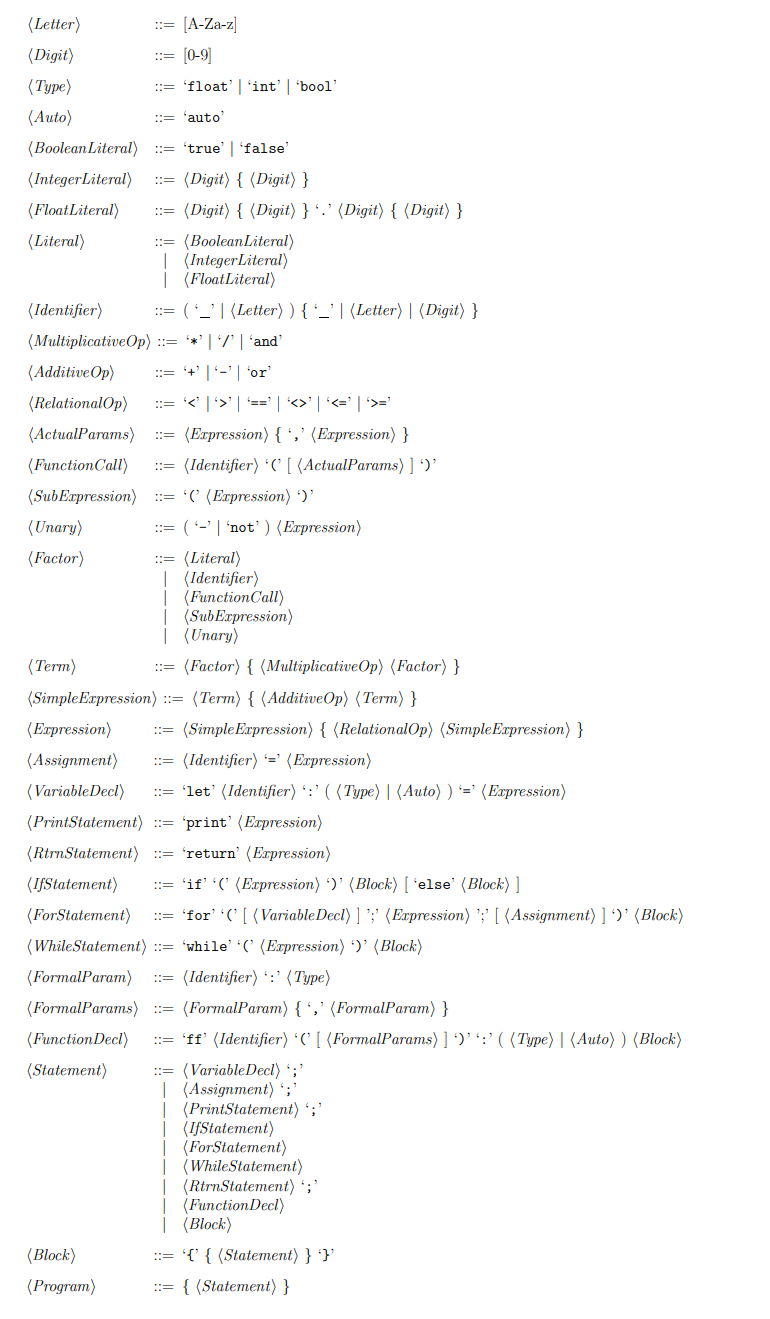
\includegraphics[width=0.6\textwidth]{smalllang.png}
			 		\centering
			  		\caption{SmallLang micro-syntax}
			  		\label{fig:smalllang}
				\end{figure}
				
				\subsection{Deterministic finite automaton}
				
				I started off by designing a DFA bit by bit, starting from the most simple classifiers such as digits. I continued building onto it by creating transitions to all states, which represent possible tokens. The DFA generated can be seen in the figure below and this was used to help in determinign whether an can be classified into a token or not. Then, from this automaton, three tables could be formed which are known as the Transition table, The Classifier table and the Token Type table.
				
				\begin{center}
					\begin{figure}[H]
			 			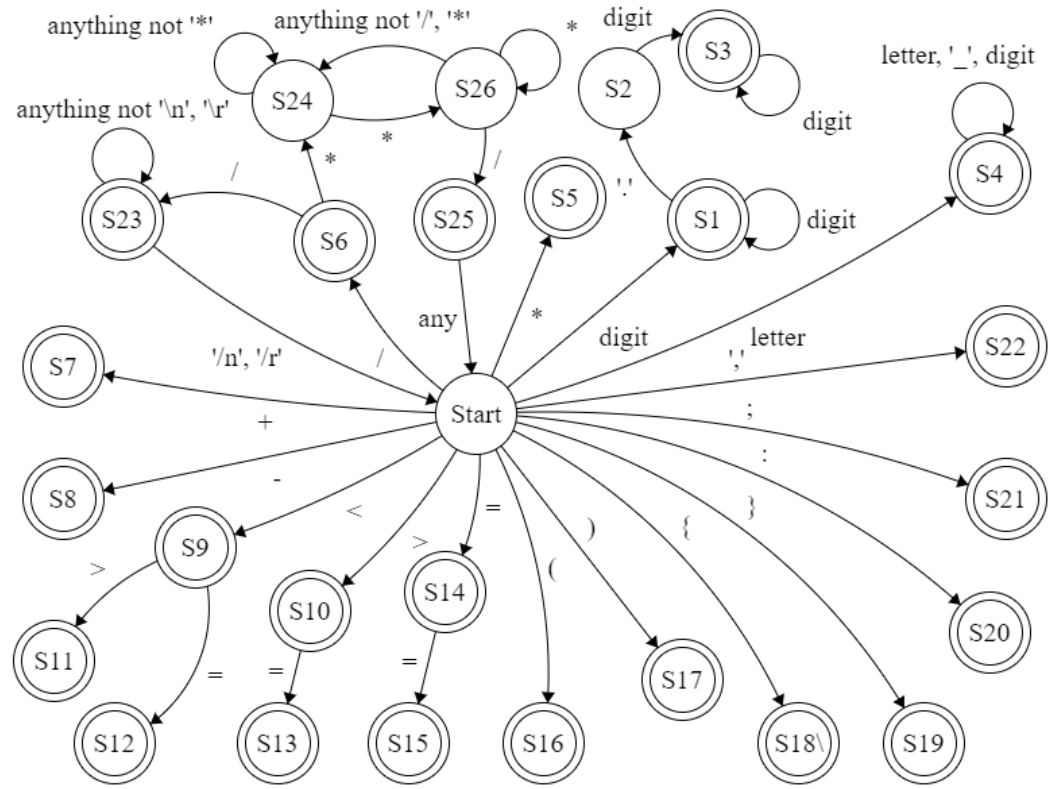
\includegraphics[width=0.9\textwidth]{automaton.png}
			 			\centering
			  			\caption{Deterministic finite automaton}
			  			\label{fig:automaton}
					\end{figure}
				\end{center}
				
				\subsection{Tables}
				
				\subsubsection{Classifier Table}
				This table shows relates the specific characters of input to the classifiers. Classifiers can also be called categories and these are then used to match them to states to create transitions as you can see in the next section. This table can be seen in the figure below.
				
				\begin{center}
					\begin{figure}[H]
			 			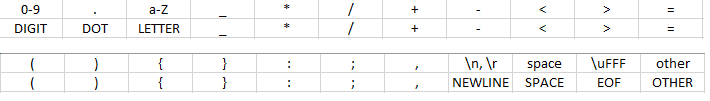
\includegraphics[width=\textwidth]{table3.png}
			  			\caption{Classifier Table}
			  			\label{fig:cat}
					\end{figure}
				\end{center}
				
				\subsubsection{Type Token Table}
				This table shows how each state is linked to a classifier. When the state is not an accepted state, it is shown as a classifier of type invalid as you can see in the figure below.
				
					\begin{center}
					\begin{figure}[H]
			 			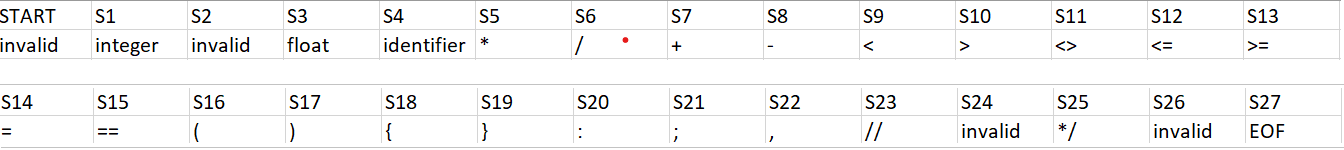
\includegraphics[width=\textwidth]{table2.png}
			  			\caption{Type Token Table}
			  			\label{fig:tokentable}
					\end{figure}
				\end{center}
				
				\subsubsection{Transition Table}
				This table shows the transitions from a state to another state when given a classifier. These are based on the automaton found in the figure above. 
				
					\begin{center}
					\begin{figure}[h!]
			 			\includegraphics[width=\textwidth]{table.png}
			  			\caption{Transition Table}
			  			\label{fig:transiitontable}
					\end{figure}
				\end{center}	
				
					\subsection{Solution}
					
					
					\subsubsection{TypeToken.java}
					
					This is an enum to hold the different types of tokens and it includes the following:
					\begin{itemize}
						\item INTEGER\_LITERAL
						\item FLOAT\_LITERAL
						\item BOOLEAN\_LITERAL
						\item IDENTIFIER
			    			\item TYPE
						\item IDENTIFIER
			    			\item AUTO
						\item IF
			    			\item FOR
						\item WHILE
			    			\item LET  
						\item PRINT
			    			\item RETURN
						\item FF
			    			\item MULTIPLICATIVE\_OP
			    			\item ADDITIVE\_OP
			    			\item RELATIONAL\_OP
						\item EQUAL\_SIGN
			    			\item BRACKET\_OPEN  
						\item BRACKET\_CLOSE
			    			\item CURLY\_OPEN
						\item CURLY\_CLOSE
			    			\item SEMI\_COLON
			    			\item COLON
			    			\item COMMA
			    			\item COMMENT\_1LINE
			    			\item COMMENT\_MULTI\_CLOSE
			    			\item EOF
			    			\item NOT
					\end{itemize}
				
				 	\subsubsection{Category.java}
					
					This is an enum to hold the different types of categories or classifiers:
					\begin{itemize}
						\item LETTER
						\item DIGIT
						\item DOT
			    			\item MULTIPLY\_OPERAND
			    			\item DIVIDE\_OPERAND
			    			\item ADDITION\_OPERAND
			    			\item SUBTRACT\_OPERAND
						\item EQUAL\_SIGN
			    			\item GT\_OPERAND  
						\item ST\_OPERAND
			    			\item BRACKET\_OPEN  
						\item BRACKET\_CLOSE
			    			\item CURLY\_OPEN
						\item CURLY\_CLOSE
			    			\item SEMI\_COLON
			    			\item COLON
			    			\item COMMA
			    			\item UNDERSCORE
			    			\item NEWLINE
			    			\item SPACE
			    			\item EOF
			    			\item OTHER
					\end{itemize}
					
				      \subsubsection{State.java}
					
					This is an enum to hold the different types of states.\\
					The states are: \textbf{START, S1, S2, S3, S4, S5, S6, S7, S8, S9, S10, S11, S12, S13, S14, S15, S16, S17, S18, S19, S20, S21, S22, S23, S24, S25, S26, S27, BAD, SE.}
					
					\subsubsection{Transition.java}
					
					This is a class which represents a transition, in fact, this class contains two members, a State holding the starting state of the transition and a Category which shows the path it needs to take. The values for these can easily be followed through from the DFA depicted in section 1.1. This class also has implementations of the overriden functions hashCode() and equals() to be able to compare these transitions later on.
			
					\subsubsection{Token.java}
					
					This is a class which represents a token and contains two members, \textbf{name (type)} and \textbf{attribute (lexeme)} which hold the token type and the identifier for that token. Apart from a constructor, this class contains the following methods.
					\begin{itemize}
						\item \textbf{getType()}: Getter for type
						\item \textbf{getAttribute()}: Getter for attribute
						\item \textbf{equals()}: Method to check if two tokens are equal
					\end{itemize}		
					
					\subsubsection{Keyword.java}
					
					This is a class which extends the Token class and in which all the keywords in the SmallLang syntax are declared. This contains \textbf{INT, FLOAT, BOOL, AUTO, IF, ELSE, FOR, WHILE, LET, RETURN, FF, PRINT, FALSE, TRUE, NOT}.	
				
					\subsubsection{Operand.java}
					
					This is a class which extends the Token class and in which all the operands in the SmallLang syntax are declared. This contains: 
					
					
					\begin{itemize}
						\item MULTIPLY (*)
						\item  DIVIDE (/)
						\item  SUBTRACT (-)
			    			\item ADDITION(+)
			    			\item AND\_OP (and)
			    			\item OR\_OP (op)
			    			\item GT (\textgreater)
						\item  LT (\textless)
			    			\item GTE (\textgreater=)
						\item  LTE (\textless=)
			    			\item  EQUAL (==)
						\item NOTEQUAL (\textless\textgreater)
					\end{itemize}
					
					\subsubsection{Lexer.java}
					
					This class contains the methods needed from the parser to obtain the next token. Firstly, this class contains these global variables which are used throughout the class:
					
					\begin{itemize}
						\item \textbf{keywords}: This is of type hashmap where the key is a string and the value is an object of type Token. This holds all the keywords and operands defined in the aforementioned name classes, Keyword and Operand.
						\item \textbf{stack}: This is a stack to hold states as the tokenization is happening.
						\item \textbf{acceptableStates}: This is of type hashmap where the key is a State and the value is an object of type TypeToken. This holds the acceptable states and their related tokentypes for example, S1 $\rightarrow$ INTEGER\_LITERAL.
						\item \textbf{currentLine}: This is of type int and is used to hold the current line in which the lexer has arrived in order to make it easier when reporting back to the user in case of errors.
			
					\end{itemize}
					
					Moreover, this class contains the methods explained below:
					
					
					\begin{enumerate}
						\item \textbf{Lexer (constructor)}: This constructor takes a parameter \textbf{filename} which is a path from the resources. Inside this function, some operations are performed to open the file into a global buffered reader. Finally, this function calls the functions \textbf{setAcceptableStates()} and  \textbf{setTransitionTable()} to initialise the lexer.
						\item \textbf{setTransitionTable()}: This function populates the transition table hashmap explained above to have all the transitions given in the automaton and transition table found in parts 1.1 and 1.2.3 respectively.
						\item \textbf{setAcceptableStates()}: This function populates the acceptable states hashmap explained above to have all the acceptable states as in the automaton and Type Token table.
						\item \textbf{getCurrentLine()}: This function would return the current line at which the reader is at.
						\item \textbf{rollback()}: This function rollbacks the reading from a file back to the marked position.
						\item \textbf{charCat()}: This function uses if statments and a switch to return the ctaegory of a particular character. This is based on the Classifier Table in section 1.2.1.
						\item \textbf{getTokens()}: This function returns an arraylist of tokens from a file input. This is used for testing.
						\item \textbf{compareTokens()}: This functon accepst two arraylists of tokens and compares them. If they are equal, true is returned, otherwise false is returned. This is also used in testing
						\item \textbf{nextToken()}: This method is called by the parser to return the next token and it uses all the aforementioned functions. 
						This function was implemented and divided into 4 steps as follows:
						\begin{enumerate}
						\item Initialisation: In this first step, the method sets the previous and current state to start, initialises a lexeme string, clears the stack and pushes the SE State into the stack. 
						\item Scanning Loop: In this step, the method loops until the state is the bad one (SE). In this loop, a character is read, the current state is checked whether it is in the list of acceptable states and if so, the stack is cleared, the current state is pushed onto the stack and the character's category is found by calling \textbf{charCat()}. Then, there are some checks for comments, and if they match, the loop continues without adding to the lexeme. However, if it is not a comment, the character obtained is added to the lexeme.
						\item Rollback Loop: After the above step, there is another loop to go on until the state is acceptable. In this loop, the state is popped and the lexeme is trimmed, resulting in an exception if there is nothing more to trim. \textbf{Rollback()} is called before doing another round to move the character pointer in the file back.
						\item Result Reporting: After all the above, the method finally reports the result. However, it first checks whether the token type is an identifier because if so, a check for a keyword is made and in this case, the keyword's Token is returned. Otherwise, a new token is returned with the tokenType associated to the current state from the \textbf{acceptableStates} hashmap together with the lexeme as attribute.
			
						
						\end{enumerate}
					\end{enumerate}
					
					
					\subsection{Testing}
					
						In order to test my implementation of this table driven lexer, I prepared some files with SmallLang code snippets, in which I made sure to target all possible types of different tokens that can be returned by the lexer. Then I wrote unit tests, which can be found in the file name \textbf{`LexerTest.java'}. These tests get a list of tokens using the \textbf{getTokens()} function explained above and compares them to a hardcoded arraylist of expected tokens to be returned by the lexer using the \textbf{compareTokens()} function. As you can see in the image below, the files containing the source files to be tested are stored in the resources folder and are named according to the part of the SmallLang syntax to be tested.
			
					\begin{figure}[h!]
			 			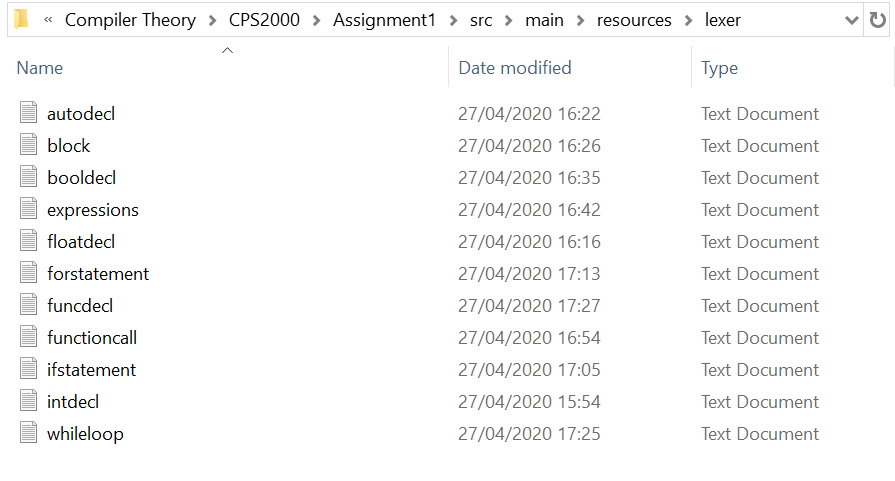
\includegraphics[width=0.8\textwidth]{testfiles.png}
			 			\centering
			  			\caption{Structure for test source files}
			  			\label{fig:lexertestfiles}
					\end{figure}
					
					
					\section{Task 2 - Hand-crafted LL parser}
					
					In this task, we were required to develop a hand-crafted predictive parser for the SmallLang language. This should interact with the aforementioned lexer through the function \textbf{nextToken()}. Moreover, this parser should be able to report any syntax errors back to the input program, while a successful parse produces an abstract syntax tree (AST) showing the structure of the input program.
					
			\noindent Furthermore, to help in the classes listed below, a \textbf{Type} enumeration with options \textbf{INT, FLOAT, BOOL} and \textbf{AUTO} was developed
					
					\subsection{AST Classes}
					
					In order to produce an abstract syntax tree, several classes were developed to be able to represent the input program in an AST. These classes can be fined in another package named \textbf{node} inside the \textbf{parser} package.
					
					\subsubsection{ASTNode.java}
					
					This is an interface with an accept method to be used later in tasks 3, 4 and 5. All the other classes implement this class.
					
					\subsubsection{ASTExpression.java}
					
					This is a class which implements the \textbf{ASTNode} interface. This is extended by other various classes as you can see further below in this section.
					
					\subsubsection{ASTStatement.java}
					
					Similarly to the class above, this is a class which implements the \textbf{ASTNode} interface and which is also extended by other classes
					
					\subsubsection{ASTProgram}
					
					This is a class which starts every program in the SmallLang language. In fact, this class only has 1 member, \textbf{statements}, which is an arraylist of objects of the type \textbf{ASTStatement}. Naturally, this includes a getter method for this member variable.
					
					\begin{figure}[H]
					\centering
			 			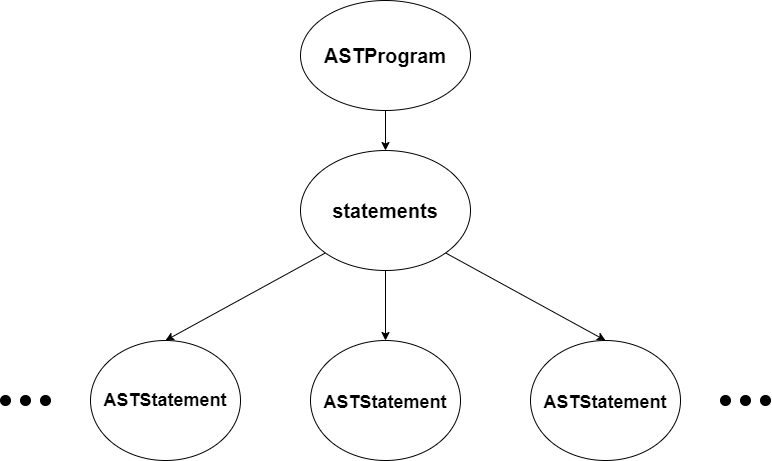
\includegraphics[width=0.55\textwidth]{astprogram.png}
			  			\caption{ASTProgram node}
			  			\label{fig:astprogram}
					\end{figure}
			
					
					
					\subsubsection{ASTIntegerLiteral}
					
					This is a class which extends the \textbf{ASTExpression} and represents an integer literal. It has one member which is \textbf{value}. Moreover, it has a constructor method and a getter for this value.
					
					
							\begin{figure}[H]
					\centering
			 			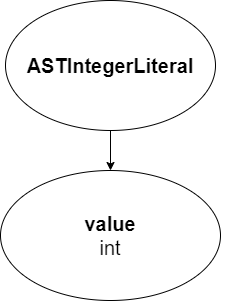
\includegraphics[width=0.25\textwidth]{astintegerlit.png}
			  			\caption{ASTIntegerLiteral node}
			  			\label{fig:astintegerlit}
					\end{figure}
					
					\subsubsection{ASTFloatLiteral}
					
					This is a class which extends the \textbf{ASTExpression} and represents a float literal. Similarly to above, it has one member which is \textbf{value}, a constructor method and a getter for this value.		
					
									\begin{figure}[H]
					\centering
			 			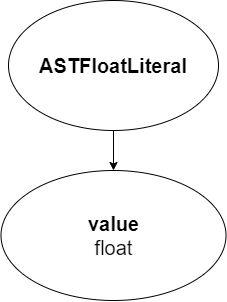
\includegraphics[width=0.25\textwidth]{astfloatlit.png}
			  			\caption{ASTFloatLiteral node}
			  			\label{fig:astfloatlit}
					\end{figure}
					
					\subsubsection{ASTBooleanLiteral}
					
					This is a class which extends the \textbf{ASTExpression} and represents a bool literal. Similarly to above, it has one member which is \textbf{value}, a constructor method and a getter for this value.		
					
									\begin{figure}[H]
					\centering
			 			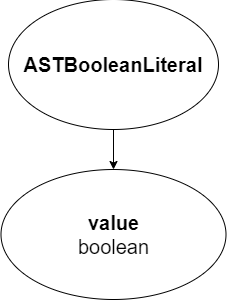
\includegraphics[width=0.25\textwidth]{astbooleanlit.png}
			  			\caption{ASTBooleanLiteral node}
			  			\label{fig:astbooleanlit}
					\end{figure}
					
					\subsubsection{ASTIdentifier}
					
					This is a class which extends the \textbf{ASTExpression} and represents an identifier. This class has the following 2 members: 
					\begin{enumerate}
					\item \textbf{value}: Its type is String and it is used to hold the variable name
					\item \textbf{type}: Its of type Type (enumeration) and it is used to hold the type of the identifier.
				
					\end{enumerate}
			In addition, this has getters for each member and a setter for the type to be used in case the identifier is of type auto so that it could be set to the expression's type as I will be explaining later.
					
					\begin{figure}[H]
					\centering
			 			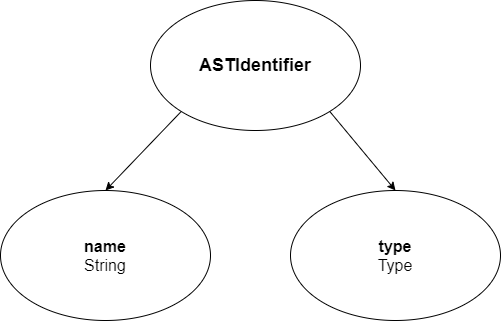
\includegraphics[width=0.55\textwidth]{astidentifier.png}
			  			\caption{ASTIdentifier node}
			  			\label{fig:astidentifier}
					\end{figure}
					
					\subsubsection{ASTBinExpression}
					Once again apart from extending \textbf{ASTExpression}, this is a class which represents a binary expression. In fact, this class has the following 3 members:
					
					\begin{enumerate}
					\item \textbf{left}: Its type is ASTExpression and it is used to hold the leftmost expression
					\item \textbf{operand}: Its of type String and it is used to hold the operator.
					\item \textbf{right}: Its type is ASTExpression and it is used to hold the rightmost expression
					\end{enumerate}
				
					 Similar to other classes, it also has getters for all members.
					 
					 
					\begin{figure}[H]
					\centering
			 			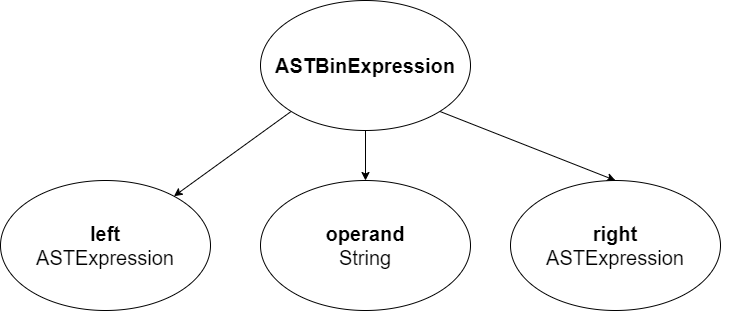
\includegraphics[width=0.65\textwidth]{astbinexpr.png}
			  			\caption{ASTBinExpression node}
			  			\label{fig:astbinexpr}
					\end{figure}
					
					\subsubsection{ASTUnary}
					This class extends \textbf{ASTExpression} and represents a unary operator `-` or `not`. Moreover, this class has two members. 		
					
					\begin{enumerate}
					\item \textbf{lexeme}: Its type is String and it is used to hold whether it is a  `-` or a `not`
					\item \textbf{expression}: Its type is ASTExpression and it is used to hold the expression after the unary operator
					\end{enumerate}
					
					 It also implements getters for these members.
					 
					\begin{figure}[H]
					\centering
			 			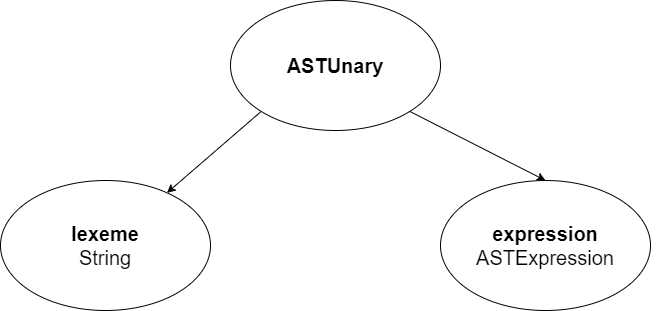
\includegraphics[width=0.6\textwidth]{astunary.png}
			  			\caption{ASTUnary node}
			  			\label{fig:astunary}
					\end{figure}
					
					\subsubsection{ASTActualParams}
					
					This is a class representing actual parameters, in fact it only consists of an arraylist of type \textbf{ASTExpression} as a member named \textbf{expressions} and its getter.
					
					\begin{figure}[H]
					\centering
			 			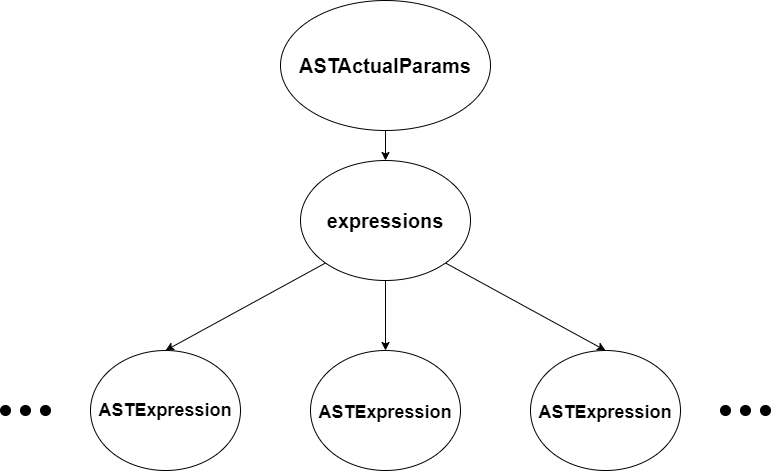
\includegraphics[width=0.6\textwidth]{astactualparams.png}
			  			\caption{ASTActualParams node}
			  			\label{fig:astactualparams}
					\end{figure}
					
					\subsubsection{ASTFunctionCall}
					
					This class also extends \textbf{ASTExpression} but represents a function call. This class has the following two members:
					
					\begin{enumerate}
					\item \textbf{identifier}: Its type is ASTIdentifier and it is used to hold the identifier of the function
					\item \textbf{params}: Its type is ASTActualParams and it is used to hold the actual parameters passed
					\end{enumerate}
					
					Just like in the other classes, we also have the getters for the members.
					
					\begin{figure}[H]
					\centering
			 			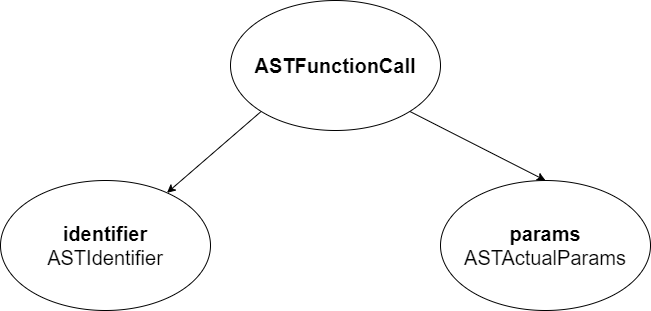
\includegraphics[width=0.6\textwidth]{astfunctioncall.png}
			  			\caption{ASTFunctionCall node}
			  			\label{fig:astfunctioncall}
					\end{figure}
						
					\subsubsection{ASTAssignment}
					
					This class extends \textbf{ASTStatement} and represents an assignment. This class has the following two members:
					\begin{enumerate}
					\item \textbf{identifier}: Its type is ASTIdentifier and it is used to hold the identifier of the variable being assigned a value
					\item \textbf{expression}: Its type is ASTExpression and it is used to hold the expression for the assignment
					\end{enumerate}	
					Just like in the other classes, we also have the getters for the members.
					
					
					\begin{figure}[H]
					\centering
			 			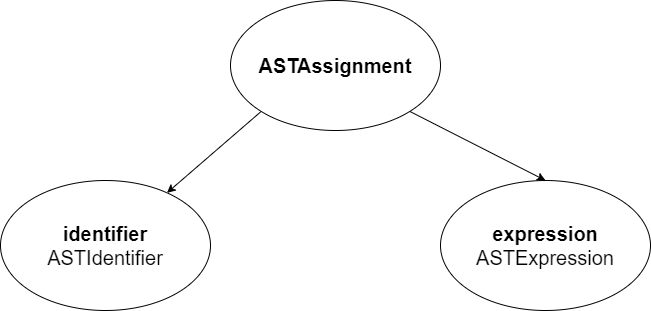
\includegraphics[width=0.6\textwidth]{astassignment.png}
			  			\caption{{ASTAssignment} node}
			  			\label{fig:astassignment}
					\end{figure}
					
					\subsubsection{ASTBlock}
					
					This class extends \textbf{ASTStatement} and represents a block. It only consists of a single member named \textbf{statements} which is an arraylist of type ASTStatement and its getter.
					
							\begin{figure}[H]
					\centering
			 			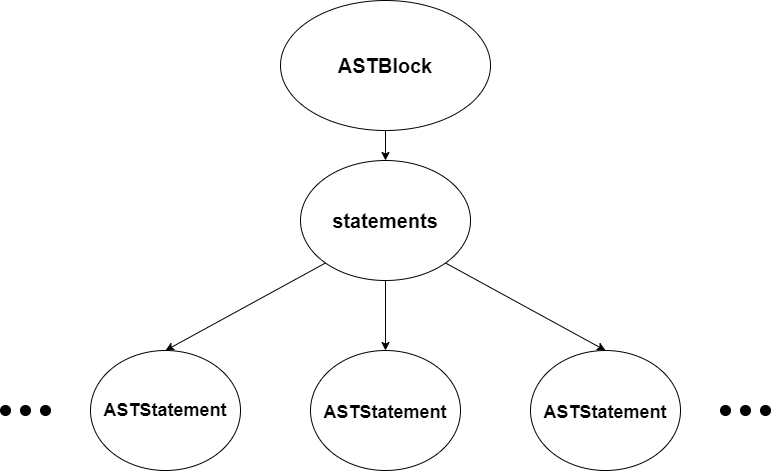
\includegraphics[width=0.55\textwidth]{astblock.png}
			  			\caption{ASTBlock node}
			  			\label{fig:astblock}
					\end{figure}
					
					\subsubsection{ASTVariableDecl}
					
					This class extends \textbf{ASTStatement} and represents a variable declaration. This class has the following two members:
					\begin{enumerate}
					\item \textbf{identifier}: Its type is ASTIdentifier and it is used to hold the identifier of the variable to declare
					\item \textbf{expression}: Its type is ASTExpression and it is used to hold the expression for the declaration
					\end{enumerate}	
					Moreover, this class also includes the getters for these members.
			
					\begin{figure}[H]
					\centering
			 			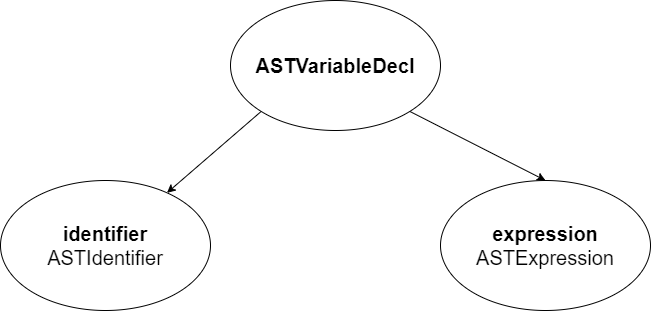
\includegraphics[width=0.55\textwidth]{astvariabledecl.png}
			  			\caption{{ASTVariableDecl} node}
			  			\label{fig:astvariabledecl}
					\end{figure}
					
					\subsubsection{ASTPrint}
					
					This class extends \textbf{ASTStatement} and represents a print statement. It consists of a member named \textbf{expression} of type ASTExpression which holds the expression to print. One can also find the getter for this expression.
			
					\begin{figure}[H]
					\centering
			 			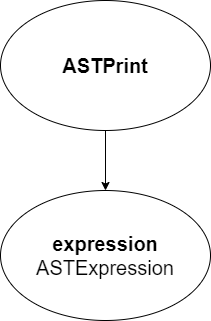
\includegraphics[width=0.25\textwidth]{astprint.png}
			  			\caption{{ASTPrint} node}
			  			\label{fig:astprint}
					\end{figure}
					 
					\subsubsection{ASTReturn}
					
					This class extends \textbf{ASTStatement} and represents a return statement. It consists of a member named \textbf{expression} of type ASTExpression which holds the expression to return. One can also find the getter for this expression.		
					
					\begin{figure}[H]
					\centering
			 			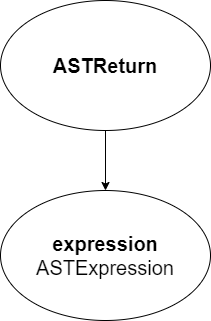
\includegraphics[width=0.25\textwidth]{astreturn.png}
			  			\caption{{ASTReturn} node}
			  			\label{fig:astreturn}
					\end{figure}	 
			
					\subsubsection{ASTIf}
					
					This class extends \textbf{ASTStatement} and represents a conditional statement. It consists of the following 3 members:
					
							\begin{enumerate}
					\item \textbf{expression}: Its type is ASTExpression and it is used to hold the expression to test as condition
					\item \textbf{block}: Its type is ASTBlock and it is used to hold the block to execute in case the expression is true
					\item \textbf{elseBlock}: Its type is ASTBlock and it is used to hold the block to execute in case the expression is false. This member can be null if there is no else condition.
					\end{enumerate}	
					This class also contains getters for these members.
					
					\begin{figure}[H]
					\centering
			 			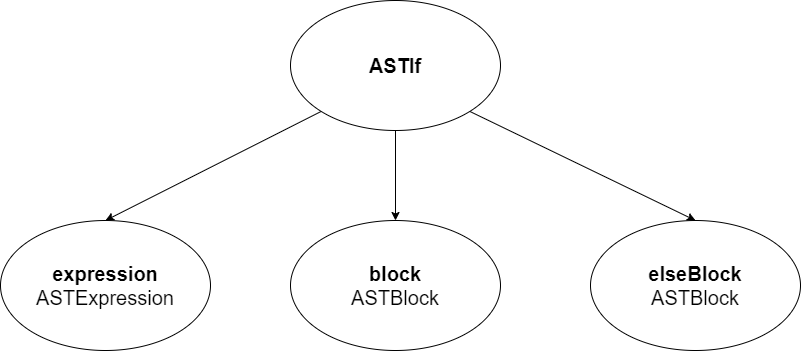
\includegraphics[width=0.65\textwidth]{astif.png}
			  			\caption{{ASTIf} node}
			  			\label{fig:astif}
					\end{figure}	 
			
						\subsubsection{ASTWhile}
					
					This class extends \textbf{ASTStatement} and represents a while loop. It consists of the following 2 members:
					
					\begin{enumerate}
					\item \textbf{expression}: Its type is ASTExpression and it is used to hold the expression to test as condition
					\item \textbf{block}: Its type is ASTBlock and it is used to hold the block to execute in case the expression is truee
					\end{enumerate}	
					
					 This class also contains getters for these members.	
					 
					 		\begin{figure}[H]
					\centering
			 			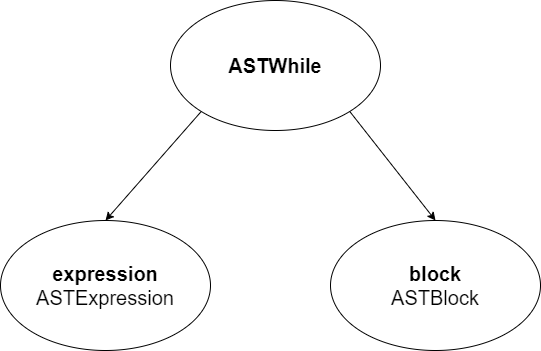
\includegraphics[width=0.55\textwidth]{astwhile.png}
			  			\caption{{ASTWhile} node}
			  			\label{fig:astwhile}
					\end{figure}	 	
				
						\subsubsection{ASTFor}
					
					This class extends \textbf{ASTStatement} and represents a for loop. It consists of the following 4 members.
					\begin{enumerate}
					\item \textbf{variableDecl}: Its type is ASTVariableDecl and it is used to hold the variable declaration which is declared in the for loop. This can be left empty and it will be null
					\item \textbf{expression}: Its type is ASTExpression and it is used to hold the expression to test as condition
					\item \textbf{assignment}: Its type is ASTAssignment and it is used to hold the assignment which is declared in the for loop. This can be left empty and it will be null
					\item \textbf{block}: Its type is ASTBlock and it is used to hold the block which is performed if the expression is true
				
					\end{enumerate}
					This class also contains all the getters for these members.
					
					\begin{figure}[H]
					\centering
			 			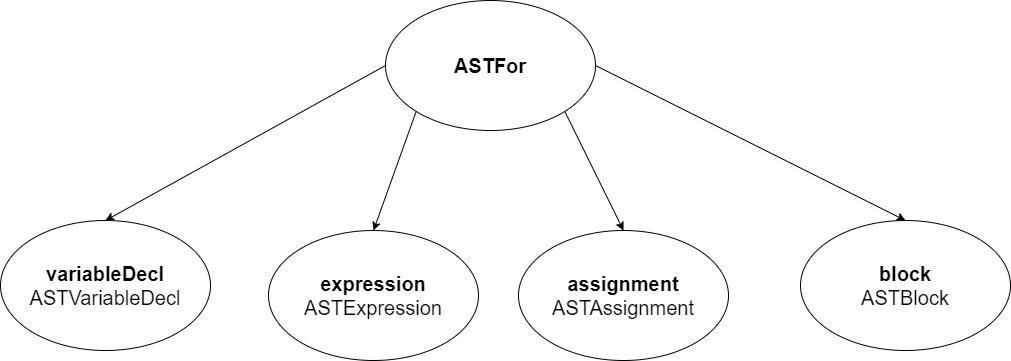
\includegraphics[width=0.7\textwidth]{astfor.png}
			  			\caption{{ASTFor} node}
			  			\label{fig:astfor}
					\end{figure}	 
					
					\subsubsection{ASTFormalParam}
					
					This class represents a formal parameter and contains only one member named \textbf{identifier} which is of type Identifier. It is an exact identifier but the type cannot be set to auto. This is checked in the constructor and if it is done, an IncorrectTypeException would be thrown. This class also has a getter for this member
					
					\begin{figure}[H]
					\centering
			 			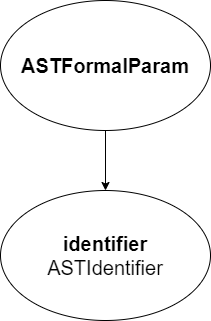
\includegraphics[width=0.25\textwidth]{astformalparam.png}
			  			\caption{{ASTFormalParam} node}
			  			\label{fig:astformalparam}
					\end{figure}	 
					
					\subsubsection{ASTFormalParams}
					
					This class represents formal parameters and contains only one member named \textbf{formalParams} which is an arraylist of ASTFormalParam. This is used by the ASTFunctionDecl class to hold its formal parameters. This class also has a getter for this member.
					
					\begin{figure}[H]
					\centering
			 			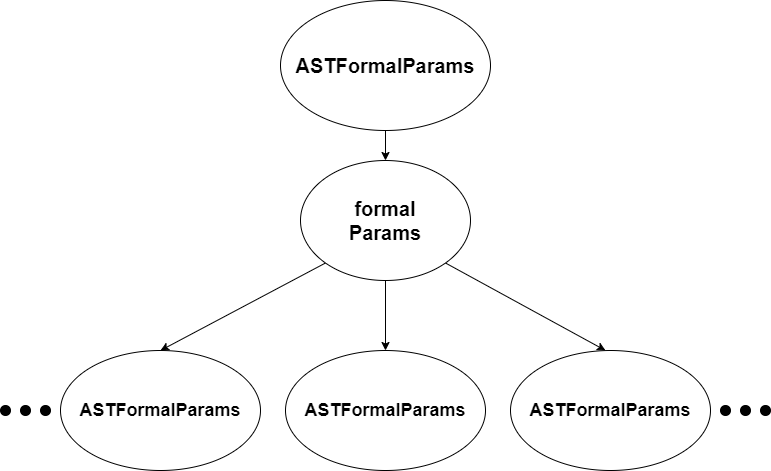
\includegraphics[width=0.7\textwidth]{astformalparams.png}
			  			\caption{{ASTFormalParams} node}
			  			\label{fig:astformalparams}
					\end{figure}	 
					
					\subsubsection{ASTFunctionDecl}
					
					This class extends \textbf{ASTStatement} and represents a function declaration. This function contains the following 3 members and its getters:
					
							\begin{enumerate}
					\item \textbf{identifier}: Its type is ASTIdentifier and it is used to hold the identifier for this new function
					\item \textbf{formalParams}: Its type is ASTFormalParams and it is used to hold the formalParams for this function
					\item \textbf{block}: Its type is ASTBlock and it is used to hold the statements which will be executed whenever this function is called
				
					\end{enumerate}
					
					\begin{figure}[H]
					\centering
			 			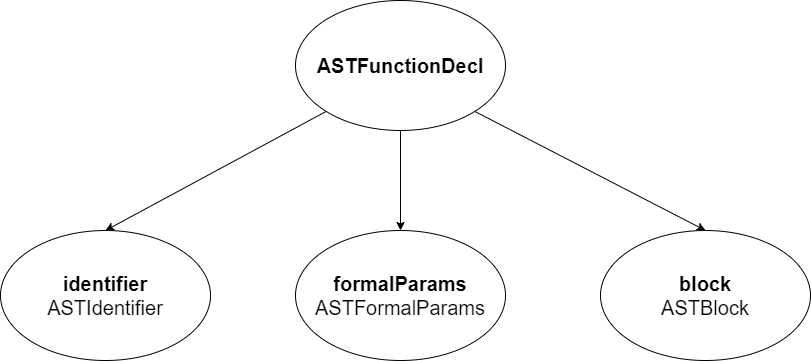
\includegraphics[width=0.55\textwidth]{astfunctiondecl.png}
			  			\caption{{ASTFunctionDecl} node}
			  			\label{fig:astfunctiondecl}
					\end{figure}	 
					
				\subsection{Solution}
				
				\subsubsection{InvalidSyntaxException}
				
				This is an exception class which extends the Exception class and it is thrown when an invalid syntax is detected by the parser. The line is also passed with the message to help the user find the error in the input program.
				
				\subsubsection{Parser.java}
				
				This is the class in which one can find methods for parsing the input program. As explained before, this works by communicating with the Lexer to request a new token after it is ready from parsing the previous one. 
				
				This class has the following two member variables:
				
				\begin{itemize}
				
				\item \textbf{lexer}: This is an object of type Lexer which is used to link a lexer to the parser. This is used by the parser to request the next token through \textbf{nextToken()}
				\item \textbf{currentToken}: This is an object of type Token and is used to hold the current token in operation.
				\end{itemize}
				
				Below, I will be explaining each method and its function in relation to how the parser works. These methods implement the micro-syntax shown in Figure \ref{fig:smalllang}.
				
				\begin{enumerate}
				\item \textbf{Parser}: This is a constructor and it initialises the parser by setting the lexer and getting the next token from it.
				\item \textbf{absorb(TypeToken)} : This is a method which checks whether the current token is of the correct type. The passed argument is the expected token and is called from the functions which I will be explaining below. If the token matches, it means syntax is valid and a new token is requested from the lexer, otherwise an InvalidSyntaxException is thrown.
				\item \textbf{literal()}: This function checks the current token and according to its type which can be either an INTEGER\_LITERAL, FLOAT\_LITERAL or a BOOLEAN\_LITERAL, it absorbs this token and then returns a new AST node according to the token type. 
				\item \textbf{identifier()}: This function is used to parse an identifier. It first absorbs a token of type IDENTIFIER and then returns a new ASTIdentifier node with the identifier name.
				\item \textbf{type()}: This function is used to parse a type. It absorbs the token of type TYPE and then returns the token being absorbed.
				
					\item \textbf{actualParams()}: This function is used to parse actual parameters. Since the syntax for a micro syntax is `\textless EXPRESSION\textgreater { ',' \textless EXPRESSION\textgreater }`, I first initialise an array list of type ASTExpression to hold expressions and check if the next token is a `)`, meaning that there are no parameters. If so, return an empty ASTActualParams object, otherwise call \textbf{expression()} to get the expression node, add it to the array list. As long as the next token type is a COMMA, I absorb the comma, get and store another expression and keep on doing so until the next token type is not a COMMA. Finally, an ASTActualParams node is returned with the collected expressions.
					
					
				\item \textbf{functionCall(ASTIdentifier)}: This function is used to parse a function call and it takes an ASTIdentifier as a parameter. Since the syntax for a micro syntax is `\textless EXPRESSION\textgreater '(' [\textless ACTUALPARAMS\textgreater] `)`, I first absorb an opening bracket token. Then, I check if the next token is a closing bracket, because if so, it means that there are no actual parameters, hence, and empty ASTActualParams node is stored. If not, it means that there are parameters and \textbf{actualParams()} is called to store them. Finally, the closing bracket is absorbed and a new ASTFunctionCall is returned with the identifier passed and the actual parameters collected.
				
					\item \textbf{unary()}: This function is used to parse a unary expression. Since the syntax for a micro syntax is `\textless EXPRESSION\textgreater ( `-` , `not` ) \textless EXPRESSION\textgreater, I first check whether the starting token is an ADDITIVE\_OP (`-`) or a NOT and absorb it. Then \textbf{expression} is called and a new ASTUnary is returned with the attribute of the ADDITIVE\_OP (`-`) or a NOT token and the expression.
						
				\item \textbf{subExpression()}: This function is used to parse a sub expression. According to the micro-syntax, a sub expression takes the form of '(' \textless EXPRESSION\textgreater ')'. Therefore, this function first absorbs an open bracket, then calls \textbf{expression()} and stores it and then absorbs the closing bracket. Finally the expression() of type ASTExpression is returned.
				
					\item \textbf{factor()}: This function is used to parse a factor. According to the micro-syntax, a factor can either be a LITERAL, IDENTIFIER, FUNCTIONCALL, SUBEXPRESSION or a UNARY. Therefore, this function checks for the type of token and if the token is of type:
				
				\begin{itemize}
				\item \textbf{INTEGER\_LITERAL, FLOAT\_LITERAL, BOOLEAN\_LITERAL}: it calls \textbf{literal()} and returns it.
				\item \textbf{IDENTIFIER, FUNCTIONCALL}: this can be either an actual identifier or a function call since both start with an identifier. To check which is which, I first call \textbf{identifier()} to absorb the identifier token and store the return in an ASTIdentifier object and then I check if the next token is an `(`. If it is, it must be a function call, hence, I call \textbf{functionCall()} with the identifier and return it. Otherwise, it must be an identifier so I simply return the identifier stored.
				\item \textbf{BRACKET\_OPEN}: it calls and returns \textbf{subExpression()} because if the first token is an opening bracket it must be a sub-expression.
				\item \textbf{NOT, SUBTRACT\_OP}: if not any of the above, it calls and returns \textbf{unary()} because that is the only option left from a factor.
			
			
				\end{itemize}
				
				\item \textbf{term()}: This function is used to parse a term. According to the micro-syntax, a term takes the form of \textless FACTOR\textgreater {\textless MULTIPLICATIVE OP (*, \, and)\textgreater} \textless FACTOR\textgreater. Therefore, this function calls \textbf{factor()} and stores it. Then there is a while loop which goes on as long as the current token is of type MULTIPLICATIVE\_OP. In this loop the MULTIPLICATIVE\_OP token is absorbed and the rightmost expression is obtained by calling \textbf{factor()}. The node initialised in the beginning is set to a new ASTBinExpression with the first expression as the current node, the operand taken from the MULTIPLICATE\_OP token and the rightmost expression obtained. Finally the expression node is returned.
				
					\item \textbf{simpleExpression()}: This function is used to parse a simple expression. According to the micro-syntax, a term takes the form of \textless TERM\textgreater {\textless ADDITIVEOP( +, -, 'or')\textgreater} \textless TERM\textgreater. Therefore, this function calls \textbf{term()} and stores it. Then there is a while loop which goes on as long as the current token is of type ADDITIVE\_OP. In this loop the ADDITIVE\_OP token is absorbed and the rightmost expression is obtained by calling \textbf{term()}. The node initialised in the beginning is set to a new ASTBinExpression with the first expression as the current node, the operand taken from the ADDITIVE\_OP token and the rightmost expression obtained. Finally the expression node is returned.
			
						\item \textbf{expression()}: This function is used to parse a simple expression. According to the micro-syntax, a term takes the form of \textless SIMPLEEXPR\textgreater {\textless RELATIONALOP(<, >, ==, <>, <=, >=)\textgreater} \textless SIMPLEEXPR\textgreater. Therefore, this function calls \textbf{simpleExpression()} and stores it. Then there is a while loop which goes on as long as the current token is of type RELATIONAL\_OP. In this loop the RELATIONAL\_OP token is absorbed and the rightmost expression is obtained by calling \textbf{simpleExpression()}. The node initialised in the beginning is set to a new ASTBinExpression with the first expression as the current node, the operand taken from the RELATIONAL\_OP token and the rightmost expression obtained. Finally the expression node is returned.
			
				\item \textbf{assignment()}: This function is used to parse an assignment. According to the micro-syntax, a term takes the form of \textless IDENTIFIER\textgreater `=` \textless EXPRESSION\textgreater. This function starts by checking if the current token is an identifier, because in the case of a for loop without an assignment, an empty ASTAssignment node has to be returned. Otherwise, the identifier is obtained by calling \textbf{identifier()}, the EQUAL\_SIGN token is absorbed and the expression is obtained by calling \textbf{expression()}. Finally, a new ASTAssignment object is returned with the identifier and expression obtained.
							
				\item \textbf{variableDeclaration()}: This function is used to parse a variable declaration. According to the micro-syntax, a term takes the form of 'let' \textless IDENTIFIER\textgreater `:` ( \textless TYPE\textgreater | \textless AUTO\textgreater ) `=`\textless EXPRESSION\textgreater. This function starts by checking if the current token is an identifier, because in the case of a for loop without an assignment, an empty ASTVariableDecl node has to be returned. Otherwise, the LET token is absorbed, the identifier is obtained by calling \textbf{identifier()} and a COLON token is absorbed. Then, we check whether it is an TYPE or AUTO and absorb it and then we set the type of the identifier. The last two steps involve absorbing the EQUAL\_SIGN token and getting the expression by calling \textbf{expression()} before returning an ASTVariableDecl object with the identifier and expression.
				
				\item \textbf{formalParam()}: This function is used to parse a variable declaration. According to the micro-syntax, a term takes the form of \textless IDENTIFIER\textgreater `:` \textless TYPE\textgreater . This function starts by obtaining an identifier by calling \textbf{identifier()}, absorbing a COLON and then obtaining the type by calling \textbf{type()}. Then, then we set the type of the identifier before returning an ASTFormalParam object with the identifier.		
				
						\item \textbf{formalParams()}: This function is used to parse formal parameters. Since the syntax for formal parameters is `\textless FORMALPARAM\textgreater { ',' \textless FORMALPARAM\textgreater }`, I first initialise an array list of type ASTFormalParam to hold params and check if the next token is a `)`, meaning that there are no parameters. If so, return an empty ASTFormalParams object, otherwise call \textbf{formalParam()} to get the parameter node, add it to the array list. As long as the next token type is a COMMA, I absorb the comma, get and store another parameter and keep on doing so until the next token type is not a COMMA. Finally, an ASTFormalParams node is returned with the collected expressions.
							
						\item \textbf{functionDeclaration()}: This function is used to parse formal parameters. The syntax for a function declaration is `ff``\textless IDENTIFIER\textgreater `(` [ \textless FORMALPARAMS\textgreater]  `)` `:` ( \textless TYPE\textgreater | \textless AUTO\textgreater ) `=`\textless EXPRESSION\textgreater. I first absorb the FF token, then I obtain an identifier by calling \textbf{identifier()} and then absorb a `(` token. The next steps include obtaining formal parameters by calling `formalParams()`, absorbing a COLON token, absorbing a toke of type AUTO or TYPE and then set the identifier's type accordingly. Finally, I obtain the block by calling \textbf{block()} and return a new ASTFunctionDecl object with the identifier, formal parameters and block obtained.
			
						\item \textbf{printStatement()}: This function is used to parse a print statement. The syntax for a print is `print``\textless EXPRESSION\textgreater, therefore a PRINT token is absorbed and an expression is obtained by calling \textbf{expression()}. Finally a new ASTPrint object with the expression is returned.			
				
						\item \textbf{returnStatement()}: This function is used to parse a return statement. The syntax for a return is `return``\textless EXPRESSION\textgreater, therefore a RETURN token is absorbed and an expression is obtained by calling \textbf{expression()}. Finally a new ASTREturn object with the expression is returned.					
						
						\item \textbf{returnStatement()}: This function is used to parse a return statement. The syntax for a return is `return``\textless EXPRESSION\textgreater, therefore a RETURN token is absorbed and an expression is obtained by calling \textbf{expression()}. Finally a new ASTREturn object with the expression is returned.	
						
						\item \textbf{ifStatement()}: This function is used to parse an if statement. The syntax for a an if statement is `if` `(` \textless EXPRESSION\textgreater `)` \textless BLOCK\textgreater [ `else` \textless BLOCK\textgreater ]. This is done by absorbing an IF token, then absorbing a `(` token, obtaining an expression by calling \textbf{expression()}, absorbing a `)` and obtaining a block by calling \textbf{block()}. The next step is checking if there is an ELSE token. If there is, the ELSE token is absorbed and another block is obtained by recalling \textbf{block()}, otherwise the else block is left as null. Finally an ASTIf object is returned with the expression and the two objects of ASTBlock.
						
						\item \textbf{forStatement()}: This function is used to parse a for statement. The syntax for a for statement is `for` `(` [\textless VARIABLEDECL\textgreater] `;` \textless EXPRESSION\textgreater `;` [\textless ASSIGNMENT\textgreater] `)` \textless BLOCK\textgreater. To do this I first absorb a FOR token, then absorb a `(` token, then call \textbf{variableDeclaration()} to obtain a variable declaration, then absorb a SEMI\_COLON, call \textbf{expression()} to obtain an expression, absorb another SEMI\_COLON token and call \textbf{assignment()} to obtain an assignment. Finally a `)' token is absorbed and the block for the loop is obtained by calling \textbf{block()}. A new ASTFor object with variable declaration, expression, assignment and the block is returned
			
			
								\item \textbf{whileStatement()}: This function is used to parse a while statement. The syntax for a while statement is `while` `(` [\textless EXPRESSION\textgreater] `)` \textless BLOCK\textgreater. To do this I first absorb a WHILE token, then absorb a `(` token, then call \textbf{expression()} to obtain an expression, then absorb a `)' token and the block for the loop is obtained by calling \textbf{block()}. A new ASTWhile object with the expression and block is returned.
								
							\item \textbf{block()}: This function is used to parse a block. The syntax for a block is `\{` \{ \textless STATEMENT\textgreater \} `\}`. To do this I first absorb a `\{` token and then initialise an arraylist of ASTStatement. Then there is a while loop which goes on until a `\}` token is found. This loop gets a statement by calling \textbf{statement()} and adds it to the arraylist. Finally a `\}` token is absorbed and an ASTBlock object is returned with the statements.
				
					\item \textbf{statement()}: This function is used to parse a statement. According to the micro-syntax, a factor can either be a VARIABLEDECL `;`, ASSIGNMENT `;`,  PRINTSTMNT `;`, IFSTMNT, FORSTMNT,  WHILESTMNT, RETURNSTMNT `;`, FUNCTIONDECL, BLOCK.
					This is done by first intialising a toReturn variable of the type ASTStatement. Therefore, this function checks for the type of token and if the token is of type:
				
				\begin{itemize}
				\item \textbf{LET}: it calls \textbf{variableDeclaration()}, sets it to the variable and absorbs a SEMI\_COLON token.
				\item \textbf{IDENTIFIER}: it calls \textbf{assignment()}, sets it to the variable and absorbs a SEMI\_COLON token.
				\item \textbf{PRINT}: it calls \textbf{printStatement()}, sets it to the variable and absorbs a SEMI\_COLON token.
				\item \textbf{IF}: it calls \textbf{ifStatement()} and sets it to the variable.	
				\item \textbf{FOR}: it calls \textbf{forStatement()} and sets it to the variable.	
				\item \textbf{WHILE}: it calls \textbf{whileStatement()} and sets it to the variable.	
				\item \textbf{RETURN}: it calls \textbf{returnStatement()}, sets it to the variable and absorbs a SEMI\_COLON token.
				\item \textbf{FF}: it calls \textbf{functionDeclaration()} and sets it to the variable.	
				\item \textbf{CURLY\_OPEN}: it calls \textbf{block()} and sets it to the variable.	
				\item \textbf{EOF}: returns null;	
					\end{itemize}
					
				After this, the toReturn variable is returned.
				
				\item \textbf{program()}: This function is used to parse a program. The syntax for a program is  \{ \textless STATEMENT\textgreater \} . To do this I am declaring an arraylist of ASTStatement and get a statement by calling \textbf{statement()}. Then there is a while loop until statement is not null in which the statement is added to the arraylist and a new statement is obtained. finally a new ASTProgram object with the statements is returned.
				
				\item \textbf{parse()}: This function starts the parsing by calling \textbf{program()}.
				
				\item \textbf{getTypeEnum(String)}: This function returns the type in enum format when given in String.
				
				
					
								
				\end{enumerate}
				
				\subsection{Testing}
				
				The parser was tested by creating several integration tests to make sure that syntax errors are outputted when they should be. I also made sure to obtain 100\% coverage so that all possible branches and cases are covered.
				
				Such tests include the following
				
				\begin{enumerate}
				\item 
				\begin{lstlisting}
				//incorrect declaration
				let x: ? int = 3;
				\end{lstlisting}
				
				\item 
				\begin{lstlisting}
				/* try */
				let x: float = 1234.a;
				\end{lstlisting}
				
				\item 
				\begin{lstlisting}
				//no correct formal param
				ff wjiw(d): int
				{
			
				}
				\end{lstlisting}
				
				\item 
				\begin{lstlisting}
				//no brackets
				if 1==1
				{
					print 1;
				}
				\end{lstlisting}
				
				\item 
				\begin{lstlisting}
				// no semi colon
				print 1
				\end{lstlisting}
				
				\item 
				\begin{lstlisting}
				//incorrect type
				let var : wrong = 5;
				\end{lstlisting}
				
				\item 
				\begin{lstlisting}
				//while no bracket
				while 1 == 1
				{
					print 1;
				}
				\end{lstlisting}
				
				\item 
				\begin{lstlisting}
				//no ending block
				{
			    	print 1;
				\end{lstlisting}
				
				\item 
				\begin{lstlisting}
				//incorrect assignment
				x 2;
				\end{lstlisting}
				
					\item 
				\begin{lstlisting}
				//formal params auto
				ff square(x: auto)
				{
			 	   return x*x;
				}
				\end{lstlisting}
				
				
				
				\end{enumerate}
				
				These tests all gave out an InvalidSyntaxException as expected.
				
				% \bibliographystyle{ieeetr}
				% \bibliography{references}
				
			
				\section{Task 3 - AST XML Generation Pass}
				
				For this task we had to implement a visitor class to output a properly indented XML representation of the abstract syntax tree returned by the parser. I started this task by creating an interface \textbf{Visitor.java} so that then I could extend it by a new class \textbf{VisitorXMLGenerator.java}. The visitor class contains void methods named visit for each AST class created and explained in section 2.1.
				
				\subsection{Solution}
				\subsubsection{VisitorXMLGenerator.java}
				This class is used to visit each AST class and print its XML representation with indentation. To be able to do this, I am keeping a member variable of type int called indent which holds the current number of tabulations, which is incremented and decrement by specific visit methods as will be explained below.
				
				The below are the methods implemented and their function:
				
				\begin{enumerate}
				\item \textbf{getIndent()}: This method is used to return a String of tabulations according to the value stored in the member variable named \textbf{indent}. 
				\item \textbf{visit(ASTActualParams)}: This method starts by getting the indentation as a string. Then, after incrementing indent, we get the ASTActualParams node's expressions and if they are empty we print the string specifying that its empty. Otherwise, the opening tag of actual params is printed, \textbf{accept()} is called for each expression and the closing tag of actual params is printed before decrementing the indent once again.
				
					\item \textbf{visit(ASTAssignment)}: This method starts by getting the indentation as a string. Then, after incrementing indent, we get the identifier and expression of the ASTAssignment node. If the assignment is null, the assignment as an empty tag is printed. Otherwise, the opening tag of assignment is printed, \textbf{accept()} is called for the identifier and the expression and the closing tag of the assignment representation is printed before decrementing the indent once again.
			
					\item \textbf{visit(ASTBinExpression)}: This method starts by getting the indentation as a string. Then, after incrementing indent, we get the operand, left and right expression of the ASTBinExpression node.  The opening tag of expression is printed with the operand, \textbf{accept()} is called for the left and right expressions and the closing tag of the assignment representation is printed before decrementing the indent once again.		
			
					\item \textbf{visit(ASTBlock)}: This method starts by getting the indentation as a string. Then, after incrementing indent, we get the statements of the ASTBlock node.  If the statements' size is 0, the assignment as an empty tag is printed. Otherwise,  The opening tag of block is printed, \textbf{accept()} is called for every statement and the closing tag of the block representation is printed before decrementing the indent once again.	
			
					\item \textbf{visit(ASTBooleanLiteral)}: This method starts by getting the indentation as a string. Then, the xml representation of the ASTBooleanLiteral is printed with the value.
			
					\item \textbf{visit(ASTfloatLiteral)}: This method starts by getting the indentation as a string. Then, the xml representation of the ASTfloatLiteral is printed with the value.
					
					\item \textbf{visit(ASTFor)}: This method starts by getting the indentation as a string. Then, after incrementing indent, we get the variable declaration, expression, assignment and block of the ASTFor node.  The opening tag of the for loop is printed, \textbf{accept()} is called for the variable declaration, expression, assignment and block and the closing tag of the for  representation is printed before decrementing the indent once again.		
			
					\item \textbf{visit(ASTFormalParam)}: This method starts by getting the indentation as a string. Then, after incrementing indent, we get the identifier of the ASTFormalParam node.  The opening tag of the for loop is printed, \textbf{accept()} is called for the identifier and the closing tag of the for  representation is printed before decrementing the indent once again.		
					
					\item \textbf{visit(ASTFormalParams)}: This method starts by getting the indentation as a string. Then, after incrementing indent, we get the formal parameters of the ASTFormalParams node.  If the formal parameters' size is 0, the formal parameters as an empty tag is printed. Otherwise,  The opening tag of formal parameters is printed, \textbf{accept()} is called for every formal parameter and the closing tag of the block representation is printed before decrementing the indent once again.	
			
					\item \textbf{visit(ASTFunctionCall)}: This method starts by getting the indentation as a string. Then, after incrementing indent, we get the identifier and parameters of the ASTFunctionCall node. The opening tag of the function call is printed, \textbf{accept()} is called for the identifier and parameters and the closing tag of the block representation is printed before decrementing the indent once again.	
				
					\item \textbf{visit(ASTFunctionDecl)}: This method starts by getting the indentation as a string. Then, after incrementing indent, we get the identifier, formal parameters and the block of the ASTFunctionDecl node. The opening tag of the function call is printed, \textbf{accept()} is called for the identifier, the formal parameters and the block and the closing tag of the block representation is printed before decrementing the indent once again.		
			
					\item \textbf{visit(ASTIdentifier)}: This method starts by getting the indentation as a string. Then, we get the type of the ASTIdentifier node. The opening tag of the function call is printed with the type together with the closing tag.	
					
							\item \textbf{visit(ASTIf)}: This method starts by getting the indentation as a string. Then, after incrementing indent, we get the expression, block and else block of the ASTIf node. The opening tag of the function call is printed, \textbf{accept()} is called for the expression, block and else block and the closing tag of the block representation is printed before decrementing the indent once again.	
							
					\item \textbf{visit(ASTIntegerLiteral)}: This method starts by getting the indentation as a string. Then, the xml representation of the ASTIntegerLiteral is printed with the value.
					
					\item \textbf{visit(ASTPrint)}: This method starts by getting the indentation as a string. Then, after incrementing indent, we get the expression of the ASTPrint node. The opening tag of the function call is printed, \textbf{accept()} is called for the expression and the closing tag of the print representation is printed before decrementing the indent once again.
					
					\item \textbf{visit(ASTProgram)}: This method starts by getting the indentation as a string. Then, after incrementing indent, we get the statements of the ASTProgram node. The opening tag of the function call is printed, \textbf{accept()} is called for every statement and the closing tag of the program representation is printed before decrementing the indent once again.		
					
					\item \textbf{visit(ASTReturn)}: This method starts by getting the indentation as a string. Then, after incrementing indent, we get the expression of the ASTReturn node. The opening tag of the function call is printed, \textbf{accept()} is called for the expression and the closing tag of the return representation is printed before decrementing the indent once again.
			
					\item \textbf{visit(ASTUnary)}: This method starts by getting the indentation as a string. Then, after incrementing indent, I get the expression and lexeme of the ASTUnary node. The opening tag of the function call is printed with the type of unary, \textbf{accept()} is called for the expression and the closing tag of the unary representation is printed before decrementing the indent once again.
	
					\item \textbf{visit(ASTVariableDecl)}: This method starts by getting the indentation as a string. Then, after incrementing indent, I get the identifier and expression of the ASTVariableDecl node. If the identifier is null, in case of a for loop with no declaration, an empty variable declaration tag is printed. Otherwise, The opening tag of the variable declaration is printed, \textbf{accept()} is called for the identifier and expression and the closing tag of the variable declaration representation is printed before decrementing the indent once again.
					
						\item \textbf{visit(ASTWhile)}: This method starts by getting the indentation as a string. Then, after incrementing indent, we get the expression and block of the ASTWhile node. The opening tag of the function call is printed, \textbf{accept()} is called for the expression and block and the closing tag of the while representation is printed before decrementing the indent once again.
						
						\item \textbf{generate()}: This function is the entry point to generate the XML representation of the input program and it directly visits the ASTProgram function.
					
						
				\end{enumerate}
				
				
				\subsubsection{Testing}
				
				In order to test my implementation of the XML representation generator, I created several tests to make sure to test all types of representations that the SmallLang language can produce. Then, I asserted that the output from this generator is as expected.
				
				The tests conducted can be found below:
				\begin{multicols}{2}
			
			
				\begin{figure}[H]
					\centering
			 			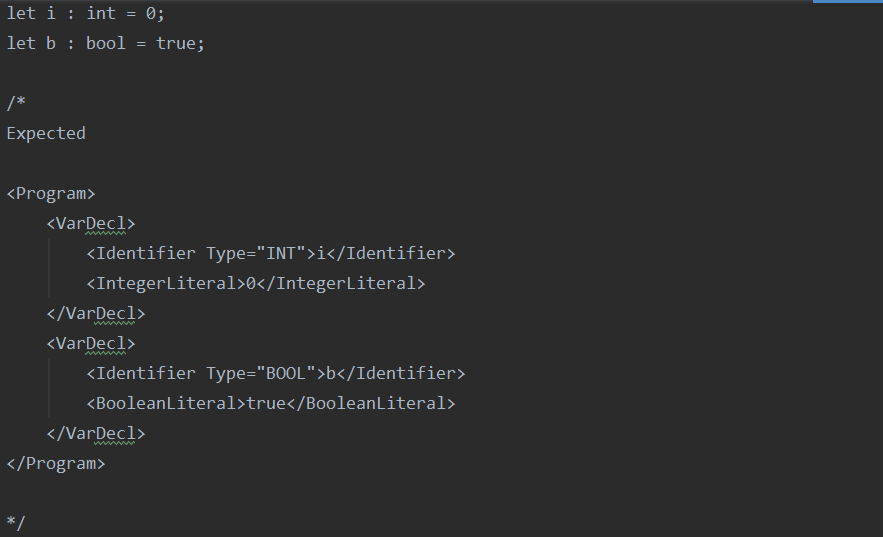
\includegraphics[width=0.45\textwidth]{xmltest1.png}
			 			\centering
			  			\caption{xmltest1.txt}
			  			\label{fig:xmltest1}
					\end{figure}
					
			\begin{figure}[H]
					\centering
			 			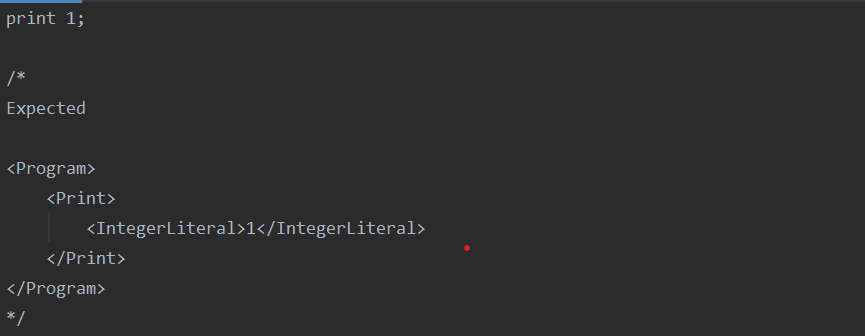
\includegraphics[width=0.45\textwidth]{xmltest2.png}
			 			\centering
			  			\caption{xmltest2.txt}
			  			\label{fig:xmltest2}
					\end{figure}
					
										
					\begin{figure}[H]
					\centering
			 			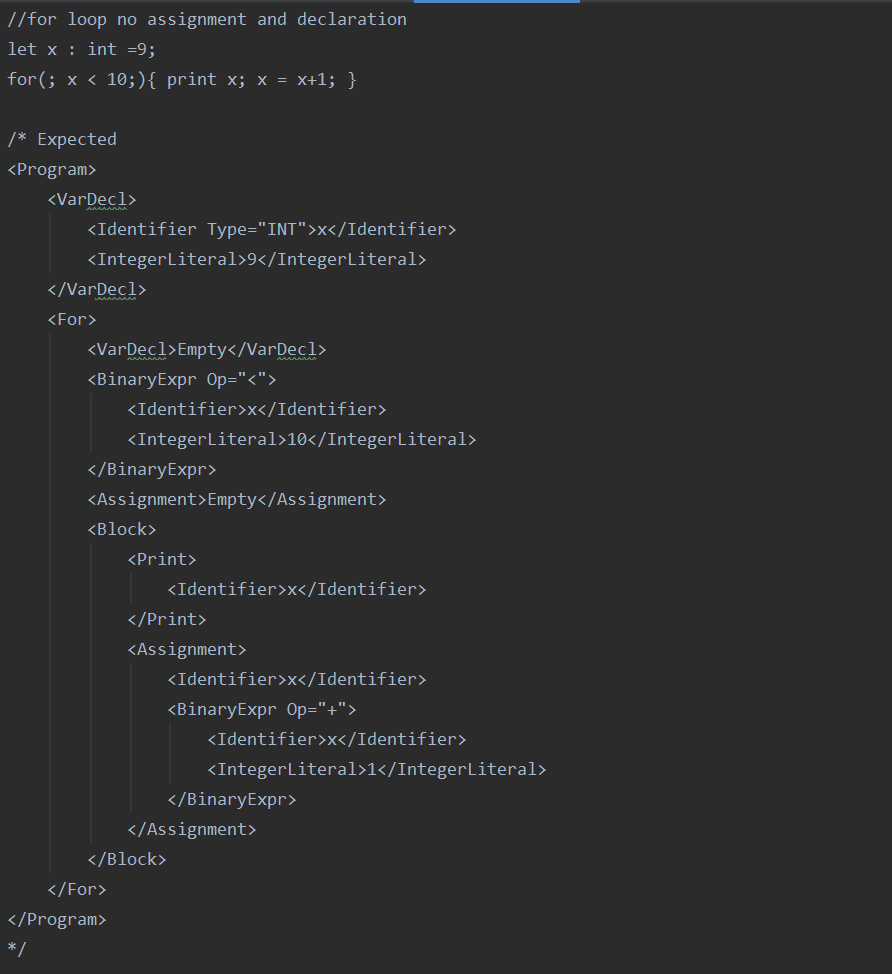
\includegraphics[width=0.45\textwidth]{xmltest9.png}
			 			\centering
			  			\caption{xmltest9.txt}
			  			\label{fig:xmltest9}
					\end{figure}
					

					
					\begin{figure}[H]
					\centering
			 			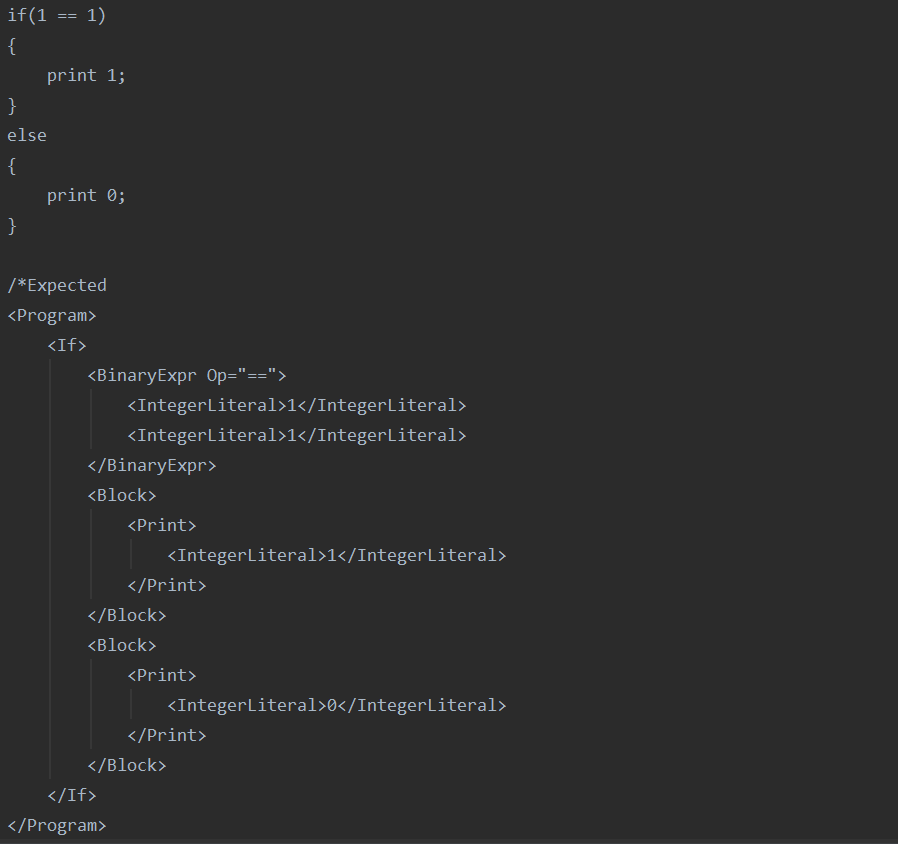
\includegraphics[width=0.45\textwidth]{xmltest4.png}
			 			\centering
			  			\caption{xmltest4.txt}
			  			\label{fig:xmltest4}
					\end{figure}
					
					\begin{figure}[H]
					\centering
			 			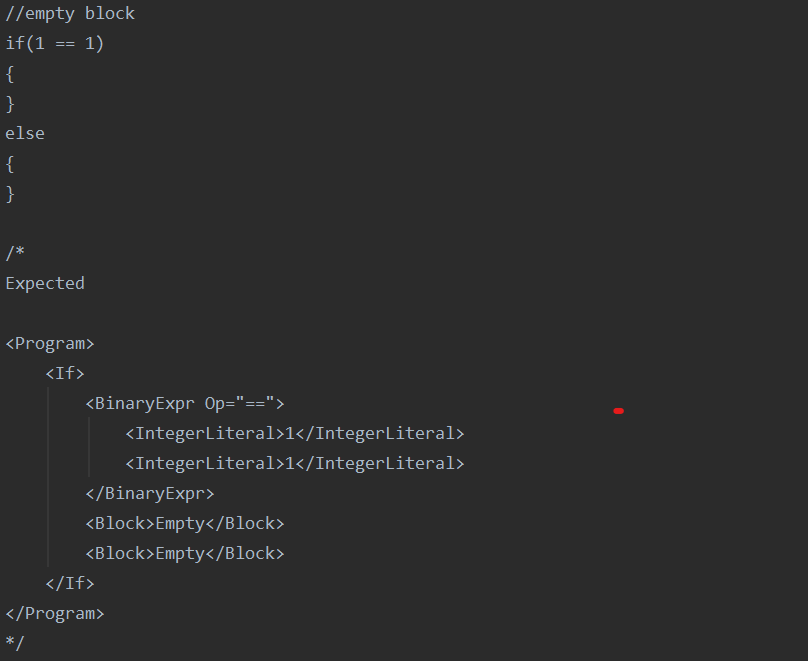
\includegraphics[width=0.45\textwidth]{xmltest5.png}
			 			\centering
			  			\caption{xmltest5.txt}
			  			\label{fig:xmltest5}
					\end{figure}
					\begin{figure}[H]
					\centering
			 			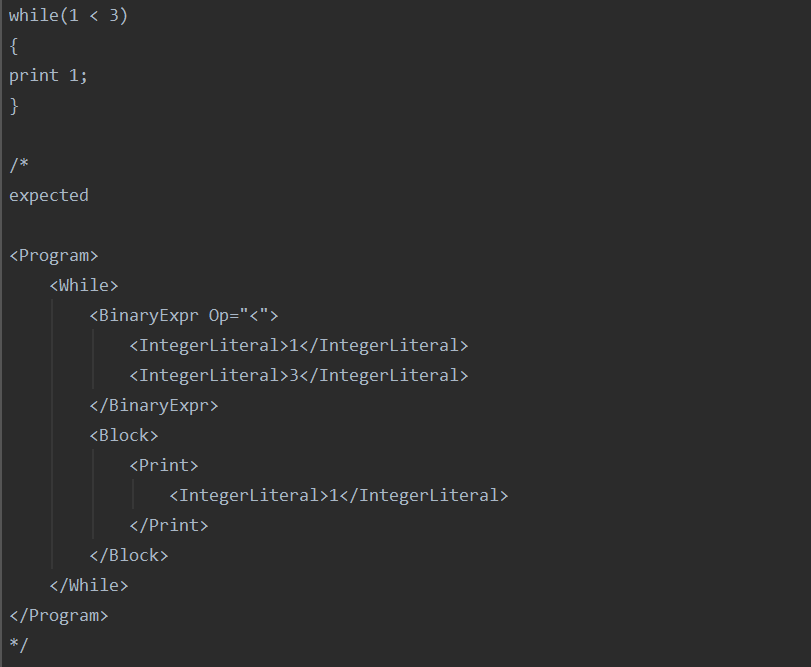
\includegraphics[width=0.45\textwidth]{xmltest6.png}
			 			\centering
			  			\caption{xmltest6.txt}
			  			\label{fig:xmltest6}
					\end{figure}
					
					\begin{figure}[H]
					\centering
			 			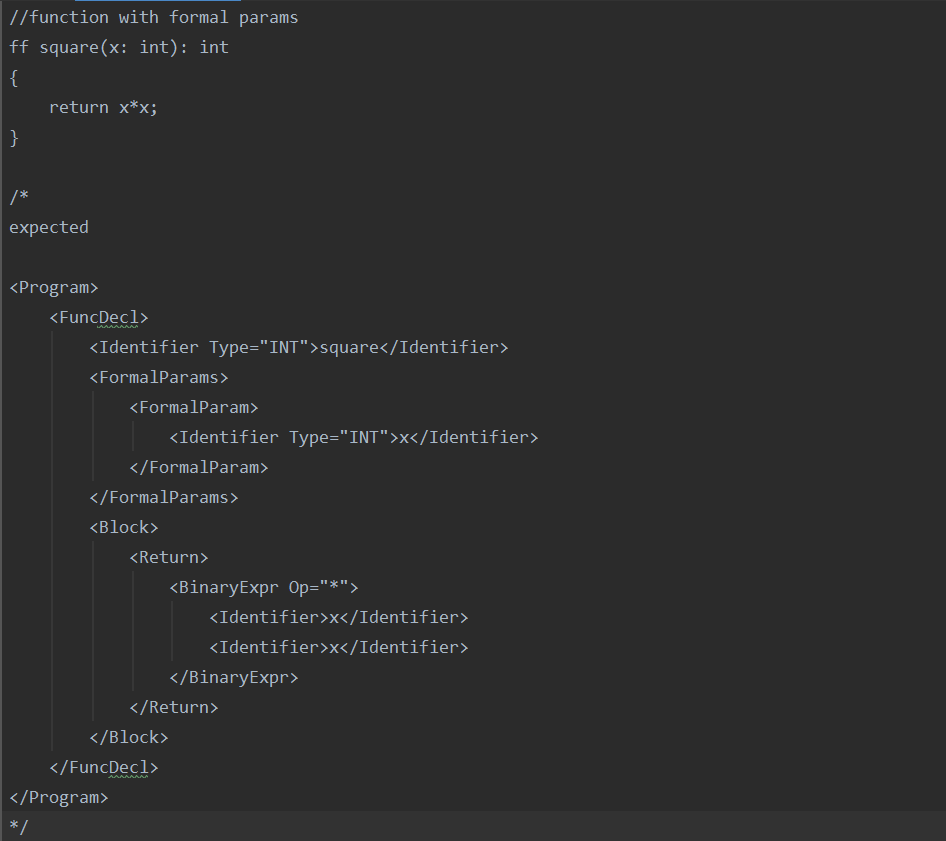
\includegraphics[width=0.45\textwidth]{xmltest7.png}
			 			\centering
			  			\caption{xmltest7.txt}
			  			\label{fig:xmltest7}
					\end{figure}
					

					
					\begin{figure}[H]
					\centering
			 			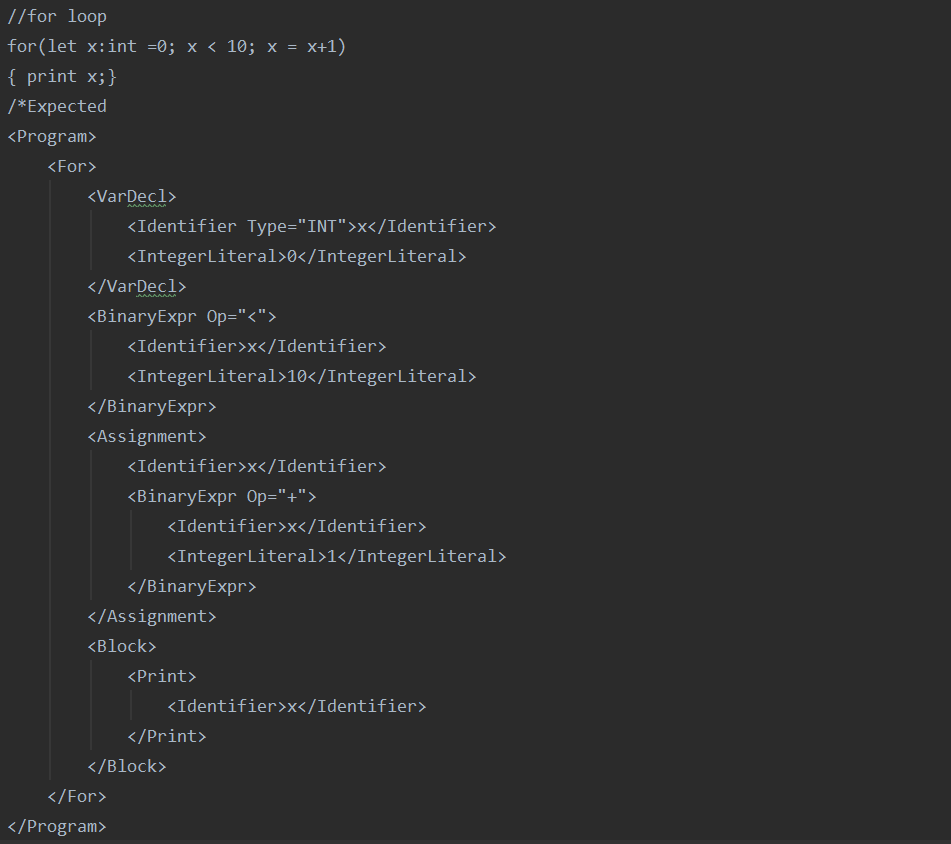
\includegraphics[width=0.45\textwidth]{xmltest8.png}
			 			\centering
			  			\caption{xmltest8.txt}
			  			\label{fig:xmltest8}
					\end{figure}

					
										\begin{figure}[H]
					\centering
			 			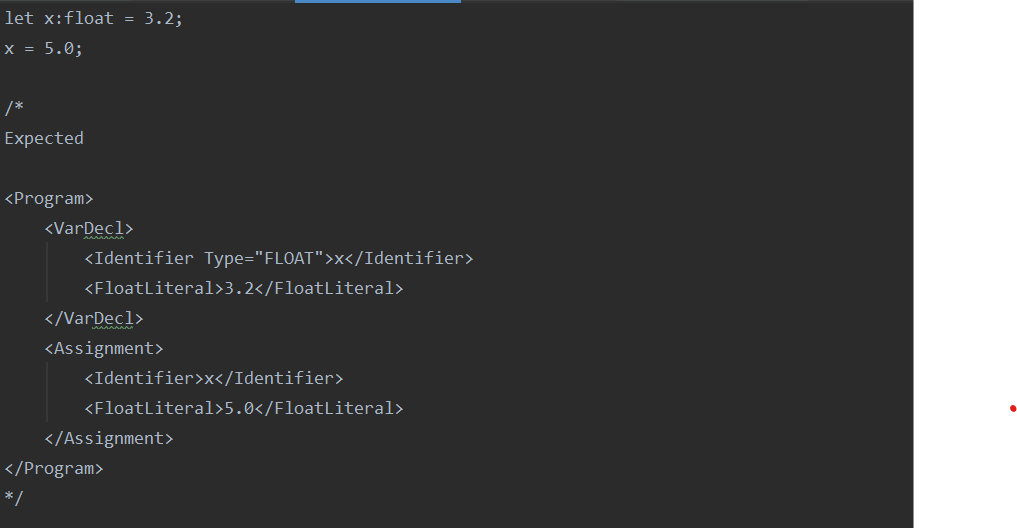
\includegraphics[width=0.45\textwidth]{xmltest3.png}
			 			\centering
			  			\caption{xmltest3.txt}
			  			\label{fig:xmltest3}
					\end{figure}
					
					
												\begin{figure}[H]
					\centering
			 			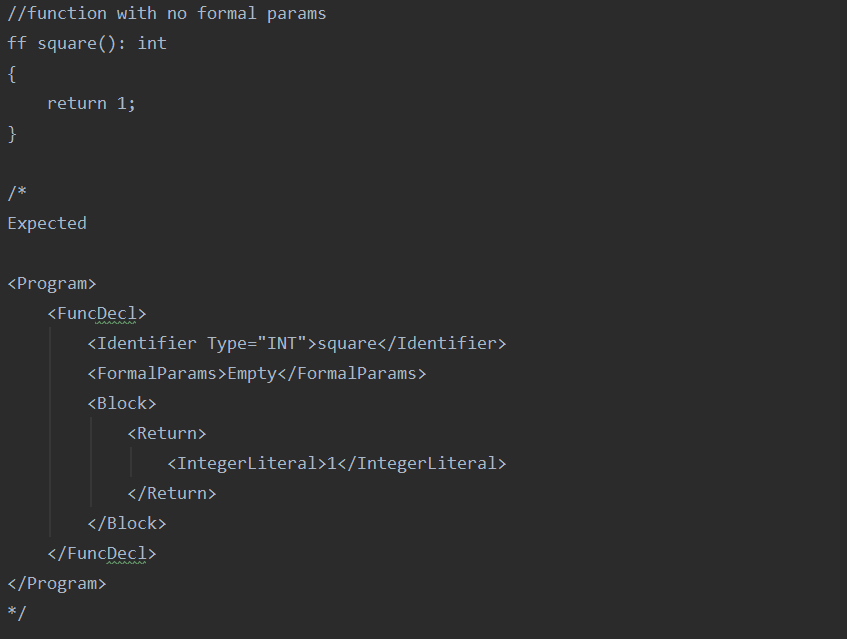
\includegraphics[width=0.45\textwidth]{xmltest10.png}
			 			\centering
			  			\caption{xmltest10.txt}
			  			\label{fig:xmltest10}
					\end{figure}
					
			
					
					\begin{figure}[H]
					\centering
			 			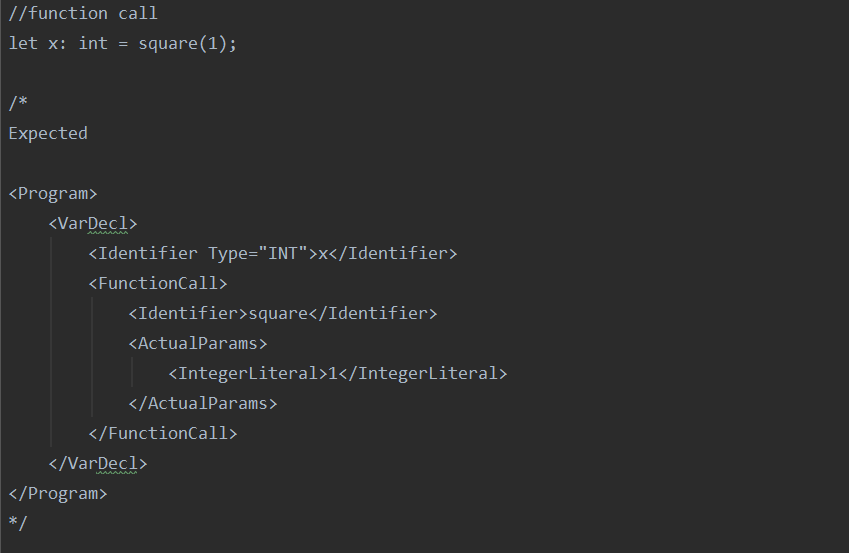
\includegraphics[width=0.45\textwidth]{xmltest11.png}
			 			\centering
			  			\caption{xmltest11.txt}
			  			\label{fig:xmltest11}
					\end{figure}
					
					\begin{figure}[H]
					\centering
			 			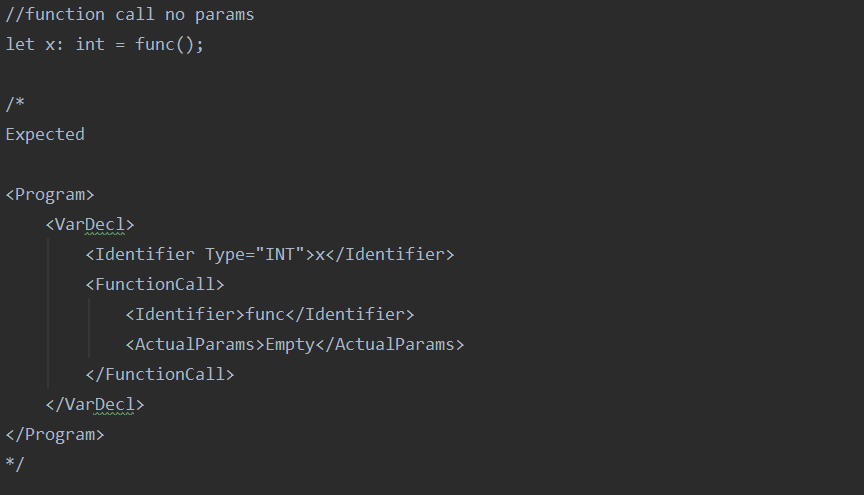
\includegraphics[width=0.45\textwidth]{xmltest12.png}
			 			 \centering
			  			\caption{xmltest12.txt}
			  			\label{fig:xmltest12}
					\end{figure}
					
					\begin{figure}[H]
					\centering
			 			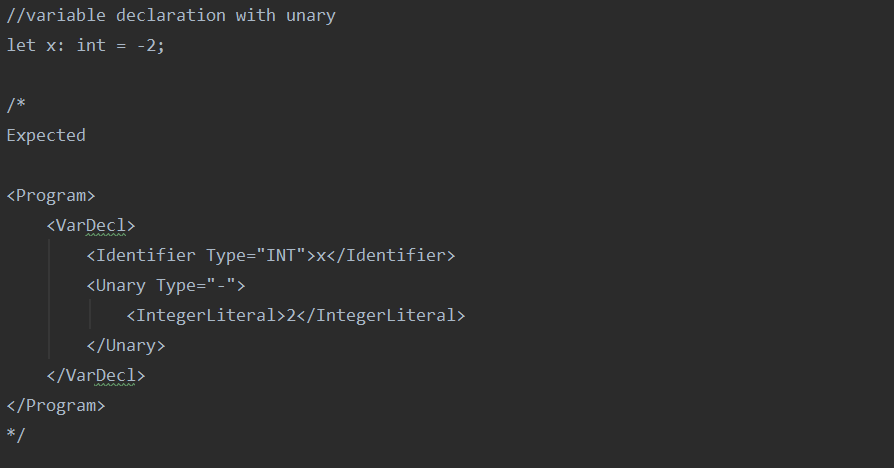
\includegraphics[width=0.45\textwidth]{xmltest13.png}
			 			\centering
			  			\caption{xmltest13.txt}
			  			\label{fig:xmltest13}
					\end{figure}
					
			\end{multicols}
			
			\section{Task 4 - Semantic Analysis Pass}
			
			In this task, another visitor class was needed to traverse the AST and perform type-checking to make sure variables are only declared once and variables are assigned to appropriate types. Moreover, a proper implementation of a symbol table was required in order to handle scopes. Finally, this semantic analyser should be able to assign types to auto variables.
			
			\subsection{Solution}
			
			\subsubsection{Scope.java}
			
			This is a class which represents a scope. This class has the following two member variables:
			\begin{itemize}
			\item \textbf{declarations}: This is a hashmap with key of type String, and the value of type ASTNode. This is used to hold declarations in the scope.
			\item \textbf{values}: This is a hashmap with key of type String, and the value of type Object. This is used to hold values for task 5.
			\end{itemize}
			
			This class contains these methods
			\begin{itemize}
			\item \textbf{Scope}: This is a simple constructor to initialise the two hashmaps
			\item \textbf{addDeclaration(String, ASTNode)}: This is a method to add a declaration to the declarations
			\item \textbf{removeDeclaration(String)}: This is a method to remove a declaration from the declarations
			\item \textbf{addValue(String, Object)}: This is a method to add a value to the values
			\item \textbf{removeValue(String)}: This is a method to remove a value from the values
			\item \textbf{getDeclarations()}: This is a function to get all the declarations of the scope
			\item \textbf{getValues()}: This is a function to get all the values of the scope
			\item \textbf{isDefined(String)}: This is a function to check if a declaration is defined.
			\end{itemize}
			
				\subsubsection{SymbolTable.java}
			
			This is a singleton class which represents a symbol table. This class has the following four member variables:
			\begin{itemize}
			\item \textbf{symbolTable}: This is a private static variable of type SymbolTable used just to make the class singleton.
			\item \textbf{scopes}: This is a Stack of Scope objects which is used to hold scopes.
			\item \textbf{constantValue}: This is a variable of type Object used to store the value from expressions. This is to be used in task 5.
			\item \textbf{constantType}: This is a variable of type Type and is used to store the constant type for expressions to be able to compare the type from one visitor method to another.
			
			\end{itemize}
			
			This class contains these methods
			\begin{itemize}
			\item \textbf{SymbolTable}: This is a simple private constructor to initialise the singleton class
			\item \textbf{getSymbolTable()}: This is a method to obtain the singleton instance of the symbol table
			\item \textbf{getScopes()}: This is a function to return the stack of scopes
			\item \textbf{getCurrentScope()}: This is a method to obtain the current scope
			\item \textbf{popScope()}: This is a function to pop a scope from the stack
			\item \textbf{insertScope(Scope)}: This is a function to insert a scope at the top of the stack
			\item \textbf{insertDecl(String, ASTNode)}: This is a function to insert a declaration to the current scope. If this identifier is already defined an \textbf{AlreadyDeclaredException} will be thrown.
			\item \textbf{insertValue(String, Object)}: This is a function to insert a value in the firsts cope where it is declared.
			\item \textbf{insertDeclGlobal(String, ASTNode)}: This is a function to insert a declaration in the global scope. %If this identifier is already defined an AlreadyDefinedException will be thrown
			\item \textbf{lookup(String)}: This is a function to search for an identifier through the loops and return it if found.
			\item \textbf{getValue(String)}: This is a function to obtain a value of an identifier where it is found first
			\item \textbf{getGlobalScope()}: This is a function to obtain the global scope
			\item \textbf{getConstantValue()}: This is a function to the value of the expression
			\item \textbf{setConstantValue(Object)}: This is a function to set the value of the expression
			\item \textbf{getConstant()}: This is a function to obtain the type of the expression
			\item \textbf{setConstant(Type)}: This is a function to set the type of the expression
			\item \textbf{reset()}: This is a function to reset the symbol table for testing purposes
			
			\end{itemize}
			
			\subsubsection{VisitorSemanticAnalysis.java}
			
			This class implements the Visitor interface and is used to visit every AST class and perform semantic analysis and throwing meaningful exceptions where needed. This class contains the following global variables:
			
					\begin{itemize}
			\item \textbf{symbolTable}: This is a variable to hold the symbol table.
			\item \textbf{functionIdentifier}: This is a variable of type ASTIdentifier to hold the current identifier for a function declaration to check the return type as I will explain further below.
			
			
			
			\end{itemize}
			
			\noindent All the visit methods implementations can be found below:
			
			\begin{enumerate}
				\item \textbf{visit(ASTActualParams)}: This method performs semantic analysis on actual parameters. This is done by getting the expressions from the ASTActualParams node and then visit each expression.
				
					\item \textbf{visit(ASTAssignment)}:This method performs semantic analysis on an assignment statement. First, we check if the expression in the node is null in case of a for loop with no assignment and if so, this is skipped. Otherwise, the expression and identifier are obtained from the node. The next step entails looking up the identifier and if this is not found in the symbol table, an \textbf{UndeclaredException} is thrown. The expression is then visited, where the expression's result type is stored in the global. After getting actual identifier's type, we check it across the type of the expression and if these do not match, an \textbf{IncorrectTypeException} is thrown. Finally the global containing the type of the expression is set to null.
			
					\item \textbf{visit(ASTBinExpression)}: This method performs semantic analysis on a binary expression node. To do this, the left and right expressions are obtained from the node. Then, the left expression is visited and the type of this expression is stored and the same is done afterwards, for the right expression. After this, the two stored types are checked and if they do not match, an \textbf{IncorrectTypeException} is thrown. The next steps involve getting the operand and operating a switch statement on it. Here, all types of operands are checked and it is made sure that they are being used with the correct types, if not,  an \textbf{IncorrectTypeException} is thrown. Finally, the type for the binary expression return is set.
			
					\item \textbf{visit(ASTBlock)}: This method performs semantic analysis on a block. This function starts by inserting a new scope and setting a variable named \textbf{alreadyReturn}, which is used to hold a flag whether there was already a return statement, to false. After this, the block's statements are obtained for every statement and it is checked if the alreadyReturn flag is set, if so a warning is outputted. Moreover, each statement is visited and if the statement is a return statement, alreayReturn is set to true. Finally, the scope is popped.
			
					\item \textbf{visit(ASTBooleanLiteral)}: This method just sets the expression's constant variable type to BOOL.
			
					\item \textbf{visit(ASTfloatLiteral)}: This method just sets the expression's constant variable type to FLOAT.
					
					\item \textbf{visit(ASTFor)}:  This method performs semantic analysis on a for statement. This is done by first getting the variable declaration from the node and visiting it, getting the expression and visiting it, getting the assignment and visiting it and finally getting and visiting the block from the ASTFor node. 
			
					\item \textbf{visit(ASTFormalParam)}: This method handles a formal parameter. This is done by getting the identifier from the ASTFormalParam node and inserting it to the declarations.
					
					\item \textbf{visit(ASTFormalParams)}: This method handles formal parameters by getting all the formal parameters from the node and visiting them one by one.
			
					\item \textbf{visit(ASTFunctionCall)}: This method performs semantic analysis on a function call. This is done by first getting the identifier and the actual identifier of the function being called by the \textbf{lookup()} method.  If the actual identifier of the function is null, meaning it was not found, an \textbf{UndeclaredException} is thrown. Then, the expressions from the ASTFunctionCall node are obtained together with the formal parameters from the function's actual identifier. The first check is done on the size of the actual parameters and the formal parameters, and if these are not equal, an \textbf{IncorrectTypeException} is thrown. After this, for each expression in the actual parameters object, the expression is visited (where the expression type is stored in the global variable), the corresponding formal parameter's type is obtained and if the expression type stored in the global and the formal parameter's type do not match, an \textbf{IncorrectTypeException} is thrown. Finally, the global variable holding the constant type is set to the type stated in the actual function's identifier declaration.
				
					\item \textbf{visit(ASTFunctionDecl)}: This method performs semantic analysis on a function declaration. This starts by removing any declarations named `return` just in case they were set before. The next step is to create a new scope to hold the actual parameters of the function declaration. The identifier of the function is obtained and stored in a variable and the formal parameters are obtained and visited. What follows is getting the block from the ASTFunctionDecl node and visiting it. If after visiting the block, there is no declaration named `return` in the symbol table, it must mean that there was no return statement and if so a \textbf{ReturnTypeMismatchException} is thrown. After this, the function declaration scope is popped and a function's identifier is inserted. \\\\
					As a point of discussion, this implementation does cover the feature to be be able to define nested function declarations, meaning other declarations inside blocks. This was only done to an extent as the lecturer advised that for the sake of this assignment, these type of programs can be used to be inexistant. This implementation does not allow a function declared inside another block to be called from outside that block because the implementation does not entail in the functions being declared in the global scope. This was not done because with the current implementation, this would pass the semantic analysis but would fail in the interpreter because as will be explained further down, the interpreter visitor method for the function declaration does not go into the block, hence, the nested function declaration is not added to the declarations, meaning when you try to call the nested function from outside the scope in which it was declared, it would not be found.
			
					\item \textbf{visit(ASTIdentifier)}: This method performs semantic analysis on an identifier by first getting the value of the identifier. This identifier is searched in the symbol table by the \textbf{lookup()} method and if it is not found, an \textbf{UndeclaredException} is thrown. Otherwise the global variable named \textbf{constantType} which holds the type for the constant expression is set to the identifier's type/
					
							\item \textbf{visit(ASTIf)}: This method performs semantic analysis on an if statement. This starts by getting the expression form the ASTIf node and visiting it. After this the true block and the else block are obtained and visited one by one.
							
					\item \textbf{visit(ASTIntegerLiteral)}:This method handles formal parameters by getting all the formal parameters from the node and visiting them one by one.
					
					\item \textbf{visit(ASTPrint)}: This method performs semantic analysis on a print statement by first getting the expression and visiting it. Finally, the constant type variable is set to null
					
					\item \textbf{visit(ASTProgram)}: This method performs semantic analysis on a program node. This is done by creating a new scope and after getting all the statements from the node, visit them one by one. Finally, the scope is popped.
					
					\item \textbf{visit(ASTReturn)}:This method performs semantic analysis on a return statement by first getting the expression and visiting it. Finally, the constant type returned from the expression is stored and checked by calling \textbf{checkReturnType()}. If this function does not throw any exceptions, the return type is stored as a declaration so that it could be used by the parent function declaration function.
			
					\item \textbf{visit(ASTUnary)}: This method performs semantic analysis on a unary expression by first getting the expression and visiting it.
										
				\item \textbf{visit(ASTVariableDecl)}: This method performs semantic analysis on a variable declaration. First, it is checked whether the expression is empty, as can happen in for loops with no variable declaration. If it is not null, the expression is obtained and visited and the identifier and the type of the identifier are obtained. If the type is auto, the type of the identifier is set to the constant type set when visiting the expression, otherwise, the type of the identifier is checked against the constant type. If these do not match, an \textbf{IncorrectTypeException} is thrown. Finally, the identifier is inserted in the scope, it is visited and the constant type is set to null.
						
						\item \textbf{visit(ASTWhile)}: his method performs semantic analysis on a while loop statement. This is done by first getting the expression and visiting it and finally, getting the block and visiting it.
	
	
						\item \textbf{analyse()}: This function is the entry point to semantically analyse the input program and it directly visits the ASTProgram function.
						
						
					\item \textbf{checkReturnType(Type)}: This function is used by return visitor method to check the return type with the function's type. This is done by getting the type of the function identifier stored in the global variable name \textbf{functionIdentifier}. If the function identifier's type is auto, the function identifier's type is set to the type passed, otherwise, the function identifier's type is checked against the type passed and if they do not match, a \textbf{ReturnTypeMismatchException} is thrown.
						
				\end{enumerate}
			
			\subsubsection{Exceptions}
			
			These are the different types of exceptions thrown by the semantic analyser
			
			\begin{enumerate}
			\item \textbf{AlreadyDeclaredException.java}: This is an exception class thrown when a variable or a function declaration is trying to be inserted but it is already declared.
			\item \textbf{UndeclaredException.java}: This is an exception class thrown when an identifier is being used but it is not yet declared.
			\item \textbf{ReturnTypeMismatchException.java}: This is an exception class thrown when a return type of a function does not match with the function's identifier type.
			\item \textbf{IncorrectTypeException.java}: This is an exception class thrown when actual parameters are not passed with the correct types, when trying to assign a variable to a wrong type or when assigning a bad type expression to an identifier on declaration.
			\end{enumerate}
			
			\subsection{Testing}
			
			Apart from the integration tests, the following tests were created to hit all the possible semantic errors that an input program can have. 
			
			\begin{enumerate}
			\item
			//incorrect type exception - expected IncorrectTypeException\\
let x:int = 3.2;
			\item
			//undeclared exception - expected UndeclaredException\\
let x:int = y;
			\item
			let x:int = 1;\\
//already declared - expected AlreadyDeclaredException\\
let x:int =2;
			\item
			//function with bad return type - expected ReturnTypeMismatchException\\
ff bad\_return\_type():int\\
\{ \\
\tab return 0.1;\\
\} \\
			\item
			//bad assignment  - expected UndeclaredException\\
x = 1;
			\item
			let x : int =1;\\
//bad assignment - expected IncorrectTypeException\\
x = 1.2;
			\item
			let x : float =1.2;\\
//bad assignment - expected IncorrectTypeException\\
x = 1;
			\item
			let x : bool =false;\\
//bad assignment - expected IncorrectTypeException\\
x = 1;
			\item
			//expression of not same types - expected IncorrectTypeException\\
let x: int = 1 + 1.2;
			\item
			//bad expression - expected IncorrectTypeException\\
let x: int = 1 and 2;
			\item
			//bad expression - expected IncorrectTypeException\\
let x: bool = true + false;
			\item
			//function call with inexistent function - expected UndeclaredException\\
let x: bool = bad\_func();
			\item
			ff plus1(x:int):int\\
 \{\\
    \tab return x+1;\\
\}\\
\\
//bad function call - expected IncorrectTypeException\\
let x: int =  plus1(1,2);
			\item
			ff plus1(x:float):float\\
 \{\\
    \tab return x+1;\\
\\\}\\\\

//bad function call - expected IncorrectTypeException\\
let x: int =  plus1(1,2);
			\item
			ff andgate(x:bool):bool\\
\{\\
    \tab return x and true;\\
\}\\\\

//bad function call - expected IncorrectTypeException\\
let x: bool =  andgate(1);
			\item
//function no return - expected ReturnTypeMismatchException\\
ff andgate(x:bool):bool\\
\{\}

			\item
//bad variable decl float - expected IncorrectTypeException\\
let x: float = 1;
			\item
//bad variable decl bool - expected IncorrectTypeException\\
let x: bool = 1;
			\item
//bad expression - expected IncorrectTypeException\\
let x: bool = true > true;
	\item
	ff square(x:int):int\\
\{\\
\tab return x*x;\\
\}\\\\
//already declared - expected AlreadyDeclaredException\\
ff square(x:int):int\\
\{\\
\tab return x*x;\\
\}\\



			\end{enumerate}
			
			
			\section{Task 5 - Interpreter Execution Pass}
			
			The last task for this assignment required another visitor class to traverse the AST and simulate an interpreter, executing the test program. The Scope class was modified at this point to also have a hashmap of values, while the symbol table was changed to have a constant value member variable apart from the aforementioned constant type member value. More details about these can be found in sections \textbf{4.1.1}
and \textbf{4.1.2}. 			

		\subsection{Solution}
		
		\subsubsection{VisitorInterpreter.java}
		
		This class implements the Visitor interface and is used to visit every AST class and perform interpretation for the statements. 
			
					\begin{itemize}
			\item \textbf{symbolTable}: This is a variable to hold the symbol table.
			
		
			\end{itemize}
			
			\noindent All the visit methods implementations can be found below:
			
			\begin{enumerate}

					\item \textbf{visit(ASTAssignment)}:This method performs interpretation on an assignment statement. First, we check if the expression in the node is null in case of a for loop with no assignment and if so, this is skipped. Otherwise, the expression and identifier are obtained from the node. The next step entails looking up the identifier and the expression is then visited, where the expression's result type and value are stored in the global variables constantValue and constantType.  Finally a new value is inserted to the hashmap of values with the value obtained from the expression with the key set to the identifier's name.
			
					\item \textbf{visit(ASTBinExpression)}: This method performs interpretation on a binary expression node. To do this, the left and right expressions are obtained from the node. Then, the left expression is visited and the type and value of this expression are stored and the same is done afterwards,  for the right expression. The next steps involve getting the operand and operating a switch statement on it. Here, for all different operands, the type stored in the global variable holding the constant type is checked and the values stored are converted either to Integer, Float or Boolean according to the type. After this, according to the operand, an operation is performed on these two values and the resulting value is set to the global symbol table variable constantValue. For division, if there is a division by 0, and Arithmetic Exception is thrown.
			
					\item \textbf{visit(ASTBlock)}: This method performs interpretation on a block. This function starts by inserting a new scope and removing any previously declared declarations with the name `return`. After this, the block's statements are obtained for every statement and each statement is visited and if after the visit, there is a declaration with the name `return`, it must mean that something was returned, hence we break out of the loop since we do not need to continue computing statements. Finally, the scope is popped.
			
					\item \textbf{visit(ASTBooleanLiteral)}: This method just sets the expression's constant variable type to BOOL and sets the value to the constantValue variable.
	
					\item \textbf{visit(ASTfloatLiteral)}: This method just sets the expression's constant variable type to FLOAT and sets the value to the constantValue variable.
					
					\item \textbf{visit(ASTFor)}:  This method performs interpretation on a for statement. This is done by first getting the variable declaration from the node and visiting it and getting the expression and visiting it. After this the value from the constantValue variable set by the expression visitor method is obtained. Then there is a while loop that goes on until the value from the expression is true. In the loop, the block from the ASTFor is obtained and visited, the assignment is obtained and visited and the expression is revisted, and the value is reset before rechecking for the loop to continue or not. So basically, this continues executing until the expression is false.
			
					\item \textbf{visit(ASTFormalParam)}: This method handles a formal parameter. This is done by getting the identifier from the ASTFormalParam node and inserting it to the declarations.
					
					\item \textbf{visit(ASTFunctionCall)}: This method performs interpretation on a function call. This is done by first getting the identifier and the actual identifier of the function being called by the \textbf{lookup()} method.   Then, the expressions from the ASTFunctionCall node are obtained together with the formal parameters from the function's actual identifier. After this, a new scope is inserted and for each expression in the actual parameters object, the expression is visited (where the expression type and value are stored in the global variable) and the value is stored in an arraylist containing the actual parameters' values. After this, all formal parameters are looped and each one is visited, its identifier is stored and a value is stored associated to the formal parameter identifier's name inside the newly created scope. After this, the block is obtained and visited before popping the newly created scope.
				
					\item \textbf{visit(ASTFunctionDecl)}: This method handles a function declaration and it only inserts a declaration for the function.
			
					\item \textbf{visit(ASTIdentifier)}: This method performs interpretation on an identifier by first getting the value of the identifier. This identifier is searched in the symbol table by the \textbf{lookup()} method. Then, I first set the type to the global variable holding the constant expression's type and then I get the value of the identifier from the values hashmap and set it to the global variable holding the constant value.
					
							\item \textbf{visit(ASTIf)}: This method performs interpretation on an if statement. This starts by getting the expression form the ASTIf node and visiting it. After this the value is obtained from the constantValue variable. If this is true, the true node is obtained and visited, otherwise, the else block is obtained and visited.
							
					\item \textbf{visit(ASTIntegerLiteral)}:This method just sets the expression's constant variable type to INT and sets the value to the constantValue variable.
					
					\item \textbf{visit(ASTPrint)}: This method performs interpretation on a print statement by first getting the expression and visiting it. Finally, the value from the variable holding the constant expression's value is printed.
					
					\item \textbf{visit(ASTProgram)}: This method performs interpretation on a program node. This is done by creating a new scope and after getting all the statements from the node, visit them one by one. Finally, the scope is popped.
					
					\item \textbf{visit(ASTReturn)}: This method performs interpretation on a return statement by first getting the expression and visiting it. Finally, the return type is stored as a declaration so that it could be used by the parent function call function.
			
					\item \textbf{visit(ASTUnary)}: This method performs interpretation on a unary expression by first getting the expression and visiting it. After visiting it, the values stored in the constantType and constantValue are stored. If the type is int, a new value is assigned to the constantValue variable by multiplying the old value to -1, else if the type is float, a new value is assigned to the constantValue variable by multiplying the old value to -1.0 or else if the 
the type is boolean, the old value is negated and a new value is set to constantValue.

				\item \textbf{visit(ASTVariableDecl)}: This method performs interpretation on a variable declaration. First, it is checked whether the expression is empty, as can happen in for loops with no variable declaration. If it is not null, the expression is obtained and visited and the identifer is also obtained. Both a declaration and a value are obtained to the symbol table and then the identifier is visited. Finally, the constant variables are set to null and the return declaration is removed in case of a function call.
						
						\item \textbf{visit(ASTWhile)}: his method performs interpretation on a while loop statement. This is done by first getting the expression and visiting it. After, the value from the expression is used as the condition for the while loop. In the while look, the block is obtained and visited and the expression of the ASTWhile node is called again and the value for the loop condition is set to the new value for rechecking whether to revisit the block.
	
	
						\item \textbf{interpret()}: This function is the entry point to interpret the input program and resets the symbol table it directly visits the ASTProgram function.
						

			\end{enumerate}
			
			\subsection{Testing}
			
			In order to test this implementation several integration tests were developed to make sure they produce expected results. This was made sure by having 100\% code coverage. Some of these test can be found below.
			
								\begin{figure}[H]
					\centering
			 			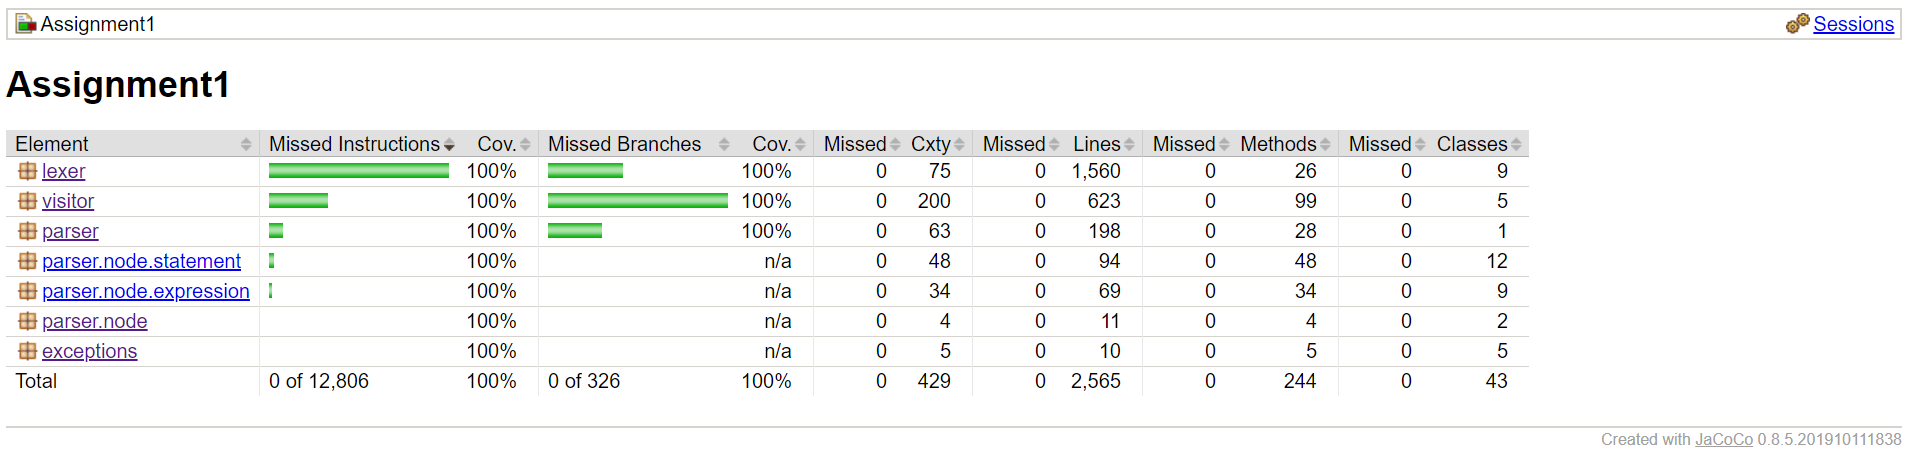
\includegraphics[width=0.8\textwidth]{jacoco.png}
			 			\centering
			  			\caption{Code Coverage}
			  			\label{fig:jacoco}
					\end{figure}
					
					\pagebreak
					
					
									\begin{multicols}{2}
			
			
				\begin{figure}[H]
					\centering
			 			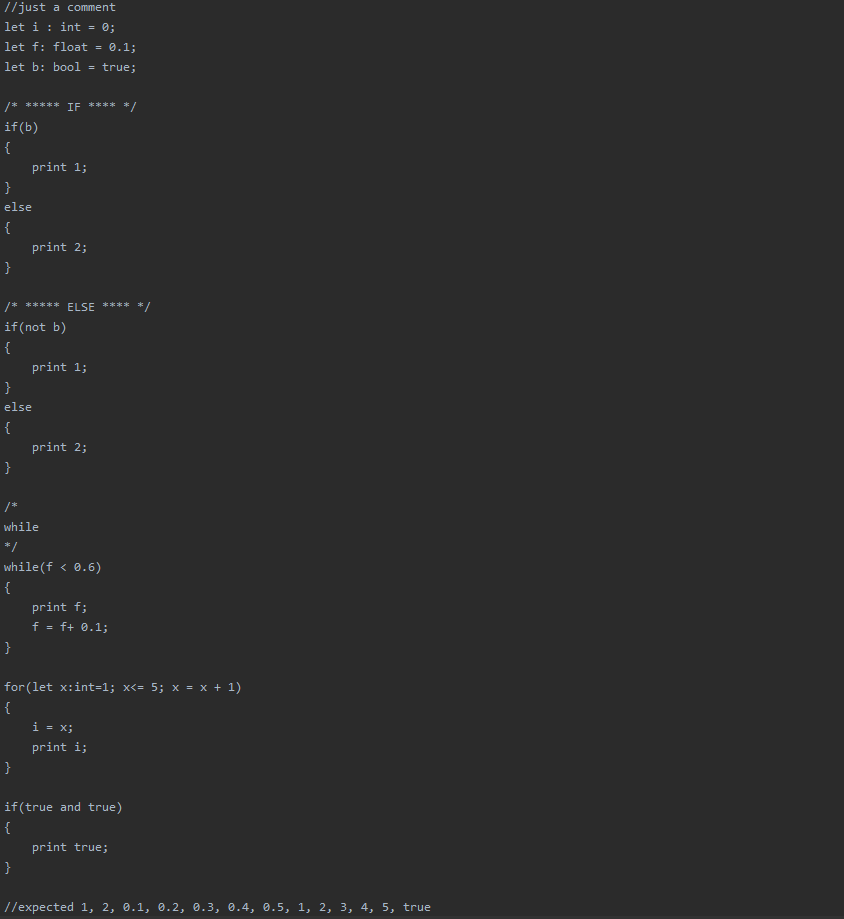
\includegraphics[width=0.45\textwidth]{test1.png}
			 			\centering
			  			\caption{test1.png}
			  			\label{fig:test1}
					\end{figure}
					
			\begin{figure}[H]
					\centering
			 			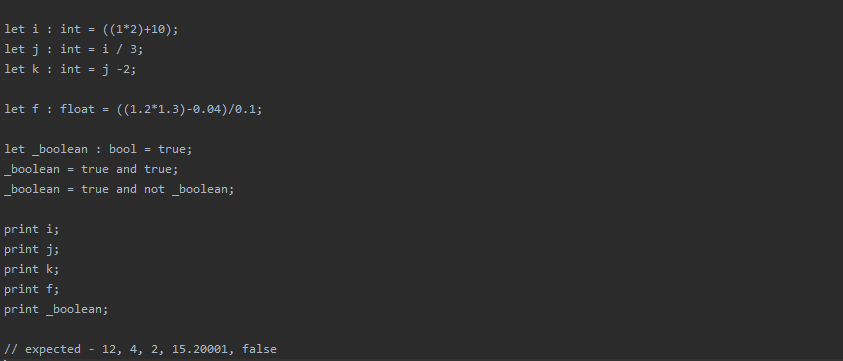
\includegraphics[width=0.45\textwidth]{test2.png}
			 			\centering
			  			\caption{test2.png}
			  			\label{fig:test2}
					\end{figure}
					
										
					\begin{figure}[H]
					\centering
			 			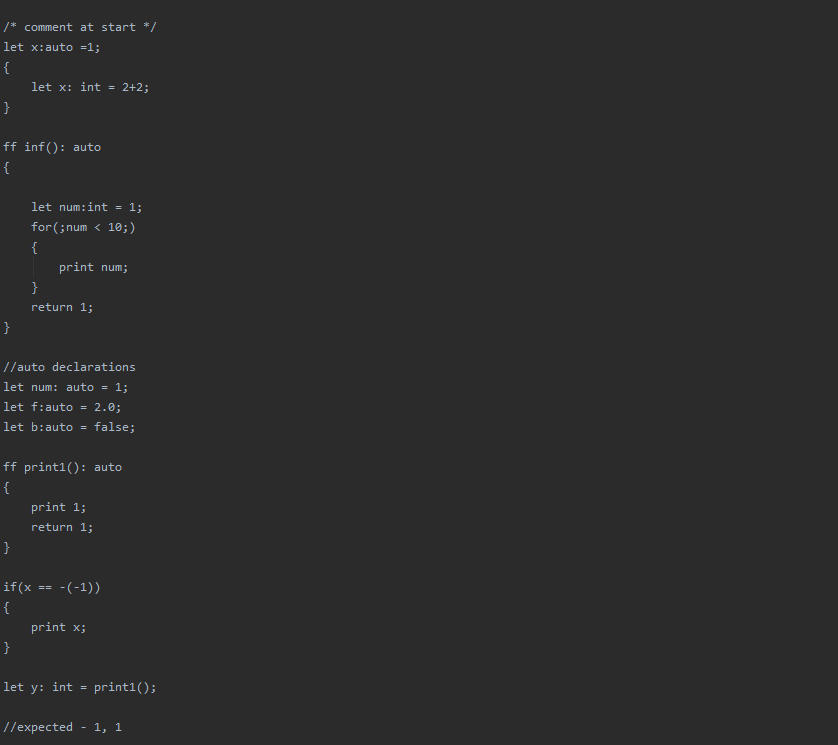
\includegraphics[width=0.45\textwidth]{test4.png}
			 			\centering
			  			\caption{test4.png}
			  			\label{fig:test4}
					\end{figure}
					
					\begin{figure}[H]
					\centering
			 			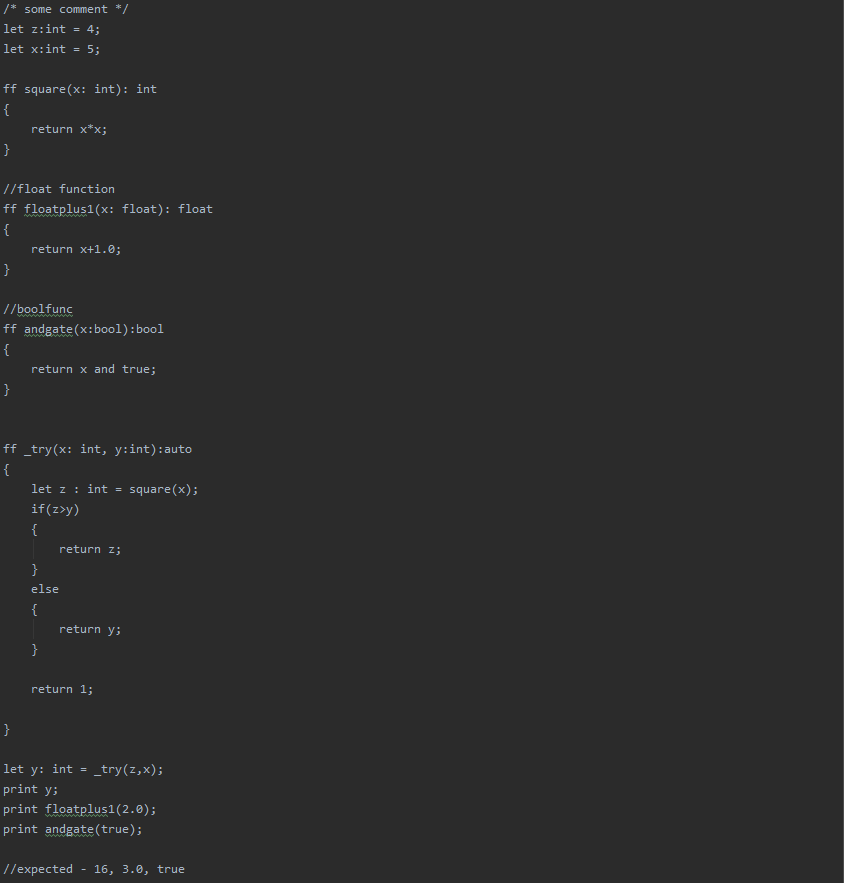
\includegraphics[width=0.45\textwidth]{test3.png}
			 			\centering
			  			\caption{test3.png}
			  			\label{fig:test3}
					\end{figure}

					

					\begin{figure}[H]
					\centering
			 			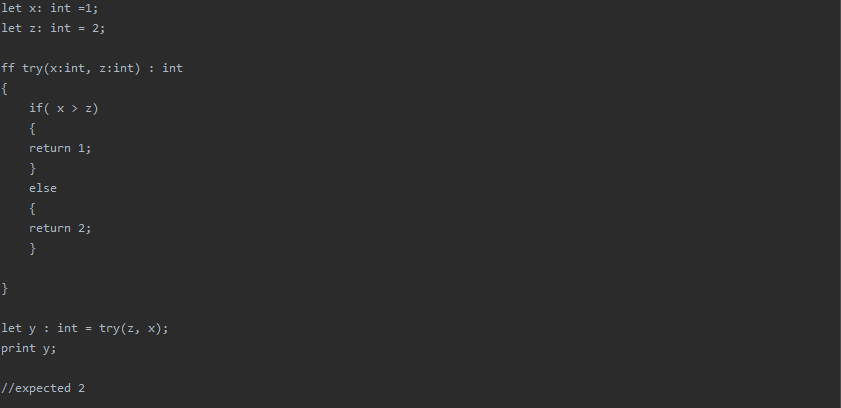
\includegraphics[width=0.45\textwidth]{test32.png}
			 			\centering
			  			\caption{test32.png}
			  			\label{fig:test32}
					\end{figure}
					
										\begin{figure}[H]
					\centering
			 			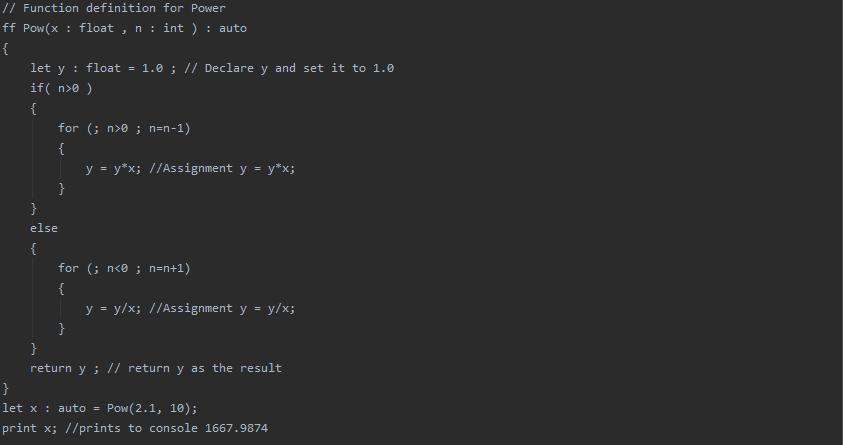
\includegraphics[width=0.45\textwidth]{test33.png}
			 			\centering
			  			\caption{test33.png}
			  			\label{fig:test33}
					\end{figure}					
			\end{multicols}
			
		
			
		
		\bibliographystyle{ieeetr}
		\nocite{*}
\bibliography{references}
			
		
			
					
			\end{document}